\documentclass[11pt,letterpaper]{article}

% PAGE FORMAT
\usepackage[letterpaper,top=3cm,bottom=3cm,left=2cm,right=2cm]{geometry}

% ENCODING AND TYPOGRAPHY
\usepackage[T1]{fontenc}
\usepackage[utf8]{inputenc}
\usepackage[spanish,es-tabla,es-nodecimaldot,es-noshorthands]{babel}
\usepackage{parskip}

% MATHEMATICS
\usepackage{amsmath,amsfonts,amssymb,amsthm}

% TABLES AND FIGURES
\usepackage{array,booktabs,multirow,longtable}
\usepackage[table]{xcolor}
\usepackage{graphicx,caption,float}

% BIBLIOGRAPHY (IEEE, escrita al final del documento)
\usepackage{cite}
\usepackage{hyperref}

\newcommand{\um}{\,\mu\mathrm{m}}
\newcommand{\uN}{\,\mu\mathrm{N}}

\title{\textbf{\LARGE Informe de avance: Influencia de la Configuración Geométrica
de una Telaraña Orbicular en su Dinámica Vibratoria
Mediante un Modelo de Mecánica Analítica}}
\author{Amelia Hoyos Vélez, Nicolle Rodríguez Estupiñán, Miguel Ángel León Botero\\[0.3cm]
\small Ingeniería Física, Escuela de Ciencias e Ingeniería, Universidad EAFIT}
\date{Semana 12 --- 2026}

\begin{document}
\maketitle

% =====================================================================
\begin{abstract}
% =====================================================================
Este informe presenta el estado del proyecto al cierre de su segundo ciclo
(semana 12 de 18). Se modela una telaraña orbicular como una red de masas
puntuales unidas por hilos elásticos pretensados y, mediante el formalismo
lagrangiano, se obtienen sus ecuaciones de movimiento linealizadas. El modelo
se implementó numéricamente para una telaraña de \textit{Araneus
diadematus} con parámetros tomados de la literatura: 28 radiales, 45 anillos
de espiral, una araña de 50 mg en el centro y 3783 grados de libertad. Se
calcularon las frecuencias naturales, los modos normales, la respuesta a un
impulso que representa una presa, la función de transferencia entre nodos y
un índice de transmisión. El modelo se verificó contra una solución
analítica y contra integración numérica directa, con errores inferiores a
$10^{-9}$. Los resultados muestran que el primer modo (2.5 Hz) corresponde al
rebote de la araña, que los modos fuera del plano dependen solo de las
pretensiones y la geometría, y que la información sobre la dirección de la
presa se concentra en la banda de 5 a 30 Hz, donde el radial de la presa
recibe entre 50 y 80 veces más señal que los demás. El avance global del
proyecto es del 66.7\,\%.
\end{abstract}

% =====================================================================
\section{Introducción}
% =====================================================================

Las arañas orbitelas, como la araña de jardín europea \textit{Araneus
diadematus}, construyen redes formadas por hilos radiales que parten de un
centro (el \emph{hub}) y una espiral de captura que los cruza. La red cumple
dos funciones a la vez: atrapa presas y funciona como un sensor. Cuando un
insecto queda atrapado, sus movimientos generan vibraciones que viajan por
los hilos hasta las patas de la araña, que permanece en el hub. A partir de
esas vibraciones la araña infiere si hay una presa, dónde está y qué tan
grande es \cite{masters1981,mortimer2016,mortimer2019decoding}.

La forma en que la vibración llega a la araña depende de la estructura de la
red: cuántos radiales tiene, cómo están espaciados los anillos de la
espiral y cuánta tensión soporta cada hilo. Estos parámetros los controla la
propia araña al construir la red, e incluso los ajusta durante la caza
\cite{nakata2010}. Esto sugiere que la geometría de la red está relacionada
con su desempeño como sensor, pero para cuantificar esa relación hace falta
un modelo físico que conecte los parámetros geométricos con la respuesta
vibratoria.

En este proyecto se construye ese modelo usando mecánica analítica. La red se
representa como un conjunto de nodos con masa unidos por hilos que se
comportan como resortes pretensados \cite{aoyanagi2010}. A partir de la
energía cinética y potencial del sistema se obtienen las ecuaciones de
movimiento, y con ellas se estudian las frecuencias naturales, las formas de
vibración y la manera en que una perturbación se transmite de un nodo a
otro.

El proyecto se organiza en tres ciclos. En el primero (semanas 1--6) se
formuló el modelo. En el segundo (semanas 7--12), que es el que reporta este
informe, el modelo se implementó numéricamente, se verificó y se usó para
caracterizar una configuración base con parámetros reales. En el tercero
(semanas 13--16) se compararán distintas geometrías.

El documento está organizado así. La sección~\ref{sec:problema} plantea el
problema y la sección~\ref{sec:objetivos} los objetivos. La
sección~\ref{sec:modelo} presenta el modelo físico con todas sus variables.
La sección~\ref{sec:metodologia} describe paso a paso cómo se resolvió
numéricamente y cómo se verificó. Las secciones~\ref{sec:resultados}
y~\ref{sec:discusion} presentan y discuten los resultados, y la
sección~\ref{sec:conclusiones} resume las conclusiones parciales. Finalmente,
la sección~\ref{sec:avance} reporta el porcentaje de avance, las dificultades
y las actividades pendientes.

% =====================================================================
\section{Planteamiento del problema}\label{sec:problema}
% =====================================================================

Cuando una presa cae sobre la red, aplica una perturbación mecánica sobre un
punto de la estructura. Esa perturbación no se queda en el punto de impacto:
se propaga por los hilos como ondas que recorren toda la red. Lo que la araña
puede inferir depende de cómo la red transforma la señal en el camino:
qué frecuencias amplifica, cuáles atenúa y cómo reparte la energía entre los
distintos radiales antes de que llegue al centro.

Esta transformación está gobernada por la mecánica de la estructura. Cada
hilo cumple dos papeles. Por un lado, se opone a ser estirado, con una fuerza
proporcional a su elongación (rigidez elástica). Por otro, como está tenso,
se opone a ser desviado lateralmente, igual que una cuerda de guitarra
(rigidez geométrica). Este segundo mecanismo es el que permite las
vibraciones perpendiculares al plano de la red.

La pregunta que guía el proyecto es:

\begin{center}
\textit{¿Cómo determina la configuración geométrica de una telaraña
orbicular sus propiedades vibratorias y la forma en que una perturbación
mecánica se transmite entre sus nodos?}
\end{center}

Para responderla se necesita: (i) un modelo que exprese la dinámica de la
red en función de su geometría, sus materiales y sus pretensiones; (ii) una
forma de calcular con él las frecuencias naturales, los modos de vibración y
la respuesta a una perturbación; y (iii) una medida cuantitativa de cuánta
señal llega desde la presa hasta la posición de la araña, que permita
comparar configuraciones distintas.

% =====================================================================
\section{Objetivos}\label{sec:objetivos}
% =====================================================================

\subsection*{Objetivo general}
Analizar la influencia de la configuración geométrica de una telaraña
orbicular en su dinámica vibratoria, mediante el modelado del sistema y el
estudio de su respuesta ante perturbaciones mecánicas, con el fin de
determinar cómo la distribución de sus nodos e hilos, así como la tensión
entre ellos, afectan las propiedades dinámicas de la estructura.

\subsection*{Objetivos específicos y estado}

\begin{table}[H]
\centering\small
\begin{tabular}{@{}p{11.5cm}p{4.5cm}@{}}
\toprule
Objetivo específico & Estado en la semana 12 \\
\midrule
OE1. Modelar la dinámica de la telaraña mediante la formulación de sus
ecuaciones de movimiento a partir de la mecánica analítica. &
Completado (ciclo 1), con ajustes en el ciclo 2. \\
OE2. Caracterizar el comportamiento vibratorio del sistema ante una
perturbación mediante sus frecuencias naturales, modos normales y
respuesta dinámica. &
Completado para la configuración base (ciclo 2). \\
OE3. Simular numéricamente la respuesta de la telaraña ante diferentes
configuraciones geométricas y perturbaciones, y contrastarla con el
análisis teórico. &
Herramienta numérica lista y verificada; comparación entre geometrías
pendiente (ciclo 3). \\
\bottomrule
\end{tabular}
\end{table}

% =====================================================================
\section{Modelo físico}\label{sec:modelo}
% =====================================================================

\subsection{Descripción de la red y nomenclatura}

La telaraña se modela en su posición de equilibrio como una estructura plana
(en el plano $z=0$) con simetría circular. Tiene $N$ hilos radiales,
igualmente espaciados en ángulo, y $M$ anillos concéntricos que representan
las vueltas de la espiral de captura. Los puntos donde un radial cruza un
anillo son los \emph{nodos} de la red. Cada nodo se identifica con un par
de índices $(n,m)$: $n=0,\dots,N-1$ indica el radial y $m=1,\dots,M$ el
anillo, contado desde el centro. Además hay un nodo central, el hub, donde
convergen todos los radiales y donde se ubica la araña, y $N$ puntos de
anclaje en el marco exterior de la red, que se consideran fijos.

Se usan tres tipos de hilo:
\begin{itemize}
    \item \textbf{Radiales:} unen el nodo $(n,m-1)$ con el $(n,m)$. El primer
    tramo ($m=1$) une el hub con el anillo 1.
    \item \textbf{Espirales:} unen el nodo $(n-1,m)$ con el $(n,m)$, es decir,
    dos radiales vecinos sobre un mismo anillo. El índice $n$ se toma módulo
    $N$, de modo que el anillo se cierra.
    \item \textbf{Anclajes:} unen cada nodo del último anillo $(n,M)$ con su
    punto fijo en el marco.
\end{itemize}

La tabla~\ref{tab:variables} reúne todas las variables del modelo.

\begin{longtable}{@{}p{2.6cm}p{10.6cm}p{2.6cm}@{}}
\caption{Variables y símbolos del modelo.}\label{tab:variables}\\
\toprule
Símbolo & Significado & Unidades \\
\midrule
\endfirsthead
\toprule
Símbolo & Significado & Unidades \\
\midrule
\endhead
\multicolumn{3}{@{}l}{\textit{Geometría}}\\
$N$ & Número de hilos radiales & --- \\
$M$ & Número de anillos de la espiral & --- \\
$n$, $m$ & Índice del radial ($0,\dots,N-1$) y del anillo ($1,\dots,M$) & --- \\
$\theta_n$ & Ángulo del radial $n$: $\theta_n=2\pi n/N$ & rad \\
$r_m$ & Radio del anillo $m$ & m \\
$\Delta$ & Separación radial entre anillos consecutivos & m \\
$R_{\text{anc}}$ & Radio del marco (puntos de anclaje) & m \\
$\mathbf{X}^0_i$ & Posición de equilibrio del nodo $i$ & m \\
$L^0_{ij}$ & Longitud de equilibrio del hilo que une los nodos $i$ y $j$ & m \\
$\hat{\mathbf{e}}^0_{ij}$ & Vector unitario del hilo $ij$, de $j$ hacia $i$ & --- \\
$\mathcal{N}(i)$ & Conjunto de nodos conectados al nodo $i$ & --- \\
\multicolumn{3}{@{}l}{\textit{Material y masas}}\\
$d_R$, $d_S$ & Diámetro de los hilos radiales y espirales & m \\
$A_{ij}$ & Área de la sección transversal del hilo: $\pi d^2/4$ & m$^2$ \\
$E_R$, $E_S$ & Módulo de Young de la seda radial (MA) y de la espiral (viscosa) & Pa \\
$\rho$ & Densidad de la seda & kg/m$^3$ \\
$\lambda_{ij}$ & Masa por unidad de longitud del hilo: $\rho A_{ij}$ & kg/m \\
$\kappa_{ij}$ & Constante elástica axial del hilo: $E A_{ij}/L^0_{ij}$ & N/m \\
$\mu_i$ & Masa concentrada en el nodo $i$ & kg \\
$m_a$ & Masa de la araña, sumada al hub & kg \\
\multicolumn{3}{@{}l}{\textit{Pretensiones}}\\
$T^0_{ij}$ & Tensión del hilo $ij$ en la posición de equilibrio & N \\
$T^R_m$ & Pretensión del tramo radial que llega al anillo $m$ ($T^R_{M+1}$: anclaje) & N \\
$T^S_m$ & Pretensión de los tramos espirales del anillo $m$ & N \\
$\bar{T}^R$ & Pretensión radial media & N \\
\multicolumn{3}{@{}l}{\textit{Dinámica}}\\
$\mathbf{u}_i(t)$ & Desplazamiento del nodo $i$ respecto al equilibrio: $(u^x_i,u^y_i,u^z_i)$ & m \\
$\boldsymbol{\delta}_{ij}$ & Desplazamiento relativo: $\mathbf{u}_i-\mathbf{u}_j$ & m \\
$\mathbf{q}(t)$ & Vector con todos los desplazamientos de los nodos libres & m \\
$T$, $V$, $\mathcal{L}$ & Energía cinética, energía potencial y lagrangiano & J \\
$\mathbf{k}^e_{ij}$ & Matriz de rigidez ($3\times3$) del hilo $ij$ & N/m \\
$\mathbf{M}$, $\mathbf{K}$ & Matrices globales de masa y de rigidez & kg, N/m \\
$\mathbf{f}(t)$ & Vector de fuerzas externas & N \\
$\omega_k$, $f_k$ & Frecuencia natural angular y en hercios del modo $k$ ($f_k=\omega_k/2\pi$) & rad/s, Hz \\
$\boldsymbol{\phi}_k$ & Forma del modo $k$ (vector propio) & kg$^{-1/2}$ \\
$\eta_k(t)$ & Coordenada modal: amplitud del modo $k$ en el tiempo $t$ & kg$^{1/2}$m \\
$p$ & Número de onda azimutal: número de oscilaciones del modo al recorrer un anillo & --- \\
$\zeta$ & Razón de amortiguamiento modal & --- \\
$F_0$ & Magnitud del impulso aplicado por la presa & N$\cdot$s \\
$\mathbf{e}_{src}$, $\mathbf{e}_{obs}$ & Vectores que seleccionan el nodo fuente (presa) y el observador & --- \\
$H_{obs,src}(\omega)$ & Receptancia: desplazamiento en el observador por unidad de fuerza en la fuente & m/N \\
$\mathcal{T}_{obs,src}$ & Índice de transmisión: integral de $|H_{obs,src}|^2$ en una banda & m$^2$/(N$^2$s) \\
\bottomrule
\end{longtable}

\subsection{Posiciones de equilibrio y grados de libertad}

En equilibrio, el nodo $(n,m)$ está en
\begin{equation}\label{eq:equil}
    \mathbf{X}^0_{n,m} = \bigl(r_m\cos\theta_n,\; r_m\sin\theta_n,\; 0\bigr),
    \qquad r_m = r_1 + (m-1)\Delta,
\end{equation}
el hub en el origen y los anclajes en
$(R_{\text{anc}}\cos\theta_n, R_{\text{anc}}\sin\theta_n, 0)$. Ante una
perturbación, cada nodo libre (el hub y los $NM$ nodos de los anillos) se
desplaza en las tres direcciones. Las componentes $u^x$ y $u^y$ describen el
movimiento \emph{en el plano} de la red y $u^z$ el movimiento
\emph{transversal}, perpendicular a ella. Reuniendo todos los
desplazamientos en un vector,
\begin{equation}\label{eq:q}
    \mathbf{q}(t)=\bigl(\mathbf{u}_{\text{hub}}^\top,\,
    \mathbf{u}_{0,1}^\top,\dots,\mathbf{u}_{N-1,1}^\top,\;\dots,\;
    \mathbf{u}_{0,M}^\top,\dots,\mathbf{u}_{N-1,M}^\top\bigr)^\top
    \in\mathbb{R}^{3(NM+1)},
\end{equation}
el sistema tiene $3(NM+1)$ grados de libertad.

\subsection{Energía cinética}

La masa de cada hilo se reparte por mitades entre sus dos extremos
\cite{meirovitch2001}, de modo que la masa del nodo $i$ es
\begin{equation}\label{eq:masas}
    \mu_i = \frac12\sum_{j\in\mathcal{N}(i)}\lambda_{ij}L^0_{ij}
    \;\bigl(+\,m_a \text{ si } i \text{ es el hub}\bigr),
\end{equation}
y la energía cinética es
\begin{equation}\label{eq:T}
    T=\frac12\sum_i \mu_i\,\dot{\mathbf{u}}_i^\top\dot{\mathbf{u}}_i .
\end{equation}

\subsection{Energía potencial}

Cuando los nodos se desplazan, la longitud del hilo $ij$ pasa de $L^0_{ij}$ a
$L_{ij}=\|\mathbf{X}^0_i-\mathbf{X}^0_j+\boldsymbol{\delta}_{ij}\|$.
Desarrollando hasta segundo orden en el desplazamiento relativo
\cite{goldstein2002},
\begin{equation}\label{eq:L2}
    L_{ij}\approx L^0_{ij}
    +\hat{\mathbf{e}}^0_{ij}\cdot\boldsymbol{\delta}_{ij}
    +\frac{1}{2L^0_{ij}}\Bigl[\|\boldsymbol{\delta}_{ij}\|^2
    -\bigl(\hat{\mathbf{e}}^0_{ij}\cdot\boldsymbol{\delta}_{ij}\bigr)^2\Bigr].
\end{equation}
El segundo término es el estiramiento del hilo a lo largo de su eje; el
tercero es el alargamiento producido por un desplazamiento perpendicular al
hilo. La energía potencial del hilo es el trabajo de la pretensión más la
energía elástica del estiramiento:
\begin{equation}\label{eq:Vhilo}
    V_{ij}= T^0_{ij}\bigl(L_{ij}-L^0_{ij}\bigr)
    +\frac12\kappa_{ij}\bigl(\hat{\mathbf{e}}^0_{ij}\cdot\boldsymbol{\delta}_{ij}\bigr)^2 .
\end{equation}
Sustituyendo \eqref{eq:L2} y sumando sobre todos los hilos se obtiene
\begin{equation}\label{eq:V}
    V=\underbrace{\sum_{(i,j)}T^0_{ij}\,\hat{\mathbf{e}}^0_{ij}\cdot\boldsymbol{\delta}_{ij}}_{\text{término lineal}}
    +\frac12\sum_{(i,j)}\boldsymbol{\delta}_{ij}^\top\mathbf{k}^e_{ij}\boldsymbol{\delta}_{ij},
\end{equation}
con la matriz de rigidez de cada hilo
\begin{equation}\label{eq:ke}
    \mathbf{k}^e_{ij}=\underbrace{\kappa_{ij}\,\hat{\mathbf{e}}^0_{ij}\hat{\mathbf{e}}^{0\top}_{ij}}_{\text{rigidez elástica}}
    +\underbrace{\frac{T^0_{ij}}{L^0_{ij}}\bigl(\mathbf{I}_3-\hat{\mathbf{e}}^0_{ij}\hat{\mathbf{e}}^{0\top}_{ij}\bigr)}_{\text{rigidez geométrica}} .
\end{equation}
El primer término actúa solo a lo largo del hilo y depende del material. El
segundo actúa en las dos direcciones perpendiculares al hilo y depende solo
de la pretensión y de la longitud: es el que da rigidez a un hilo tenso
frente a desplazamientos laterales \cite{meirovitch2001}.

\subsection{Condición de equilibrio de las pretensiones}\label{sec:equilibrio}

El término lineal de \eqref{eq:V} se puede reescribir como
$-\sum_i \mathbf{u}_i\cdot\mathbf{F}^0_i$, donde
$\mathbf{F}^0_i=\sum_{j\in\mathcal{N}(i)}T^0_{ij}\hat{\mathbf{e}}^0_{ji}$ es
la fuerza neta que las pretensiones ejercen sobre el nodo $i$. Para que la
configuración plana sea realmente de equilibrio, y para que el modelo lineal
tenga sentido, esa fuerza debe anularse en todo nodo libre:
\begin{equation}\label{eq:equilibrio}
    \sum_{j\in\mathcal{N}(i)} T^0_{ij}\,\hat{\mathbf{e}}^0_{ji} = \mathbf{0}.
\end{equation}
En el nodo $(n,m)$ actúan cuatro hilos: el radial interior tira hacia el
centro con $T^R_m$, el radial exterior tira hacia afuera con $T^R_{m+1}$, y
los dos tramos espirales tiran hacia los nodos vecinos del mismo anillo. Por
la simetría, la suma de estos dos últimos apunta hacia el centro y vale
$2T^S_m\sin(\pi/N)$. Imponiendo \eqref{eq:equilibrio} en la dirección radial:
\begin{equation}\label{eq:recurrencia}
    T^R_{m+1} = T^R_m + 2\,T^S_m\sin\!\left(\frac{\pi}{N}\right),
    \qquad m = 1,\dots,M.
\end{equation}
La pretensión radial debe crecer hacia afuera para compensar el tirón de la
espiral. Esto tiene dos consecuencias. Primera, los nodos del último anillo
necesitan un hilo que tire hacia afuera, por lo que la red debe estar anclada
a un marco. Segunda, las pretensiones no se pueden escoger libremente: una
vez fijadas $T^S_m$ y la pretensión radial media, la
recurrencia~\eqref{eq:recurrencia} determina todas las $T^R_m$. En el hub,
los $N$ radiales tiran simétricamente y su suma es cero, así que el hub
también está en equilibrio. Con \eqref{eq:equilibrio} el término lineal de
\eqref{eq:V} desaparece y la energía potencial es puramente cuadrática.

\subsection{Ecuaciones de movimiento}

Con el lagrangiano $\mathcal{L}=T-V$ y las ecuaciones de Euler--Lagrange
\begin{equation}
    \frac{\mathrm{d}}{\mathrm{d}t}\frac{\partial\mathcal{L}}{\partial\dot{\mathbf{u}}_i}
    -\frac{\partial\mathcal{L}}{\partial\mathbf{u}_i}=\mathbf{0},
\end{equation}
se obtiene, para cada nodo libre,
\begin{equation}\label{eq:eom_local}
    \mu_i\,\ddot{\mathbf{u}}_i = -\sum_{j\in\mathcal{N}(i)}\mathbf{k}^e_{ij}\bigl(\mathbf{u}_i-\mathbf{u}_j\bigr)
    + \mathbf{f}_i(t),
\end{equation}
donde $\mathbf{u}_j=\mathbf{0}$ si $j$ es un anclaje. Reuniendo todas las
ecuaciones en forma matricial,
\begin{equation}\label{eq:sistema}
    \mathbf{M}\ddot{\mathbf{q}}+\mathbf{K}\mathbf{q}=\mathbf{f}(t),
\end{equation}
donde $\mathbf{M}=\mathrm{diag}(\mu_i\mathbf{I}_3)$ y $\mathbf{K}$ se obtiene
sumando la contribución de cada hilo: el bloque $\mathbf{k}^e_{ij}$ se suma
en las posiciones $(i,i)$ y $(j,j)$ y se resta en $(i,j)$ y $(j,i)$. Si uno de
los extremos es un anclaje, solo se suma el bloque del nodo libre.
$\mathbf{K}$ es simétrica y, gracias a los anclajes, definida positiva.

\subsection{Separación entre movimiento en el plano y transversal}

Como la red en equilibrio es plana, ningún vector $\hat{\mathbf{e}}^0_{ij}$
tiene componente $z$. Según \eqref{eq:ke}, la componente $zz$ de cada
$\mathbf{k}^e_{ij}$ vale $T^0_{ij}/L^0_{ij}$ y las componentes que mezclan
$z$ con $x$ o $y$ son nulas. Por tanto, el sistema se separa exactamente en
dos problemas independientes:
\begin{equation}\label{eq:desacople}
    \mathbf{K} = \mathbf{K}_P \oplus \mathbf{K}_T,
\end{equation}
uno para el movimiento en el plano ($P$) y otro para el transversal ($T$).
Una consecuencia física importante es que los modos transversales dependen
solo de las pretensiones, las longitudes y las masas, y no del módulo de
Young de la seda. En cambio, los modos en el plano dependen de ambos.

\subsection{Análisis modal}

Las frecuencias naturales $\omega_k$ y los modos $\boldsymbol{\phi}_k$ son
las soluciones del problema de valores propios generalizado
\begin{equation}\label{eq:evp}
    \mathbf{K}\boldsymbol{\phi}_k=\omega_k^2\,\mathbf{M}\boldsymbol{\phi}_k ,
\end{equation}
con los modos normalizados de forma que
\begin{equation}\label{eq:ortog}
    \boldsymbol{\phi}_k^\top\mathbf{M}\boldsymbol{\phi}_l=\delta_{kl},\qquad
    \boldsymbol{\phi}_k^\top\mathbf{K}\boldsymbol{\phi}_l=\omega_k^2\delta_{kl}.
\end{equation}
Cada modo es una forma de vibración en la que todos los nodos oscilan a la
misma frecuencia. Por la simetría circular de la red, cada modo tiene un
número de onda azimutal $p$ que indica cuántas oscilaciones completas hace al
recorrer un anillo: $p=0$ es un modo en el que todos los radiales se mueven
igual, $p=1$ uno en el que la mitad de la red sube mientras la otra baja, y
así sucesivamente. Los modos con $p\neq0$ y $p\neq N/2$ aparecen en pares
con la misma frecuencia (pares degenerados), que son el mismo patrón girado.

\subsection{Respuesta a una perturbación}

La presa se modela como un impulso de magnitud $F_0$ aplicado en el nodo
fuente en la dirección $z$: $\mathbf{f}(t)=F_0\,\delta(t)\,\mathbf{e}_{src}$.
Expresando la respuesta como superposición de modos,
$\mathbf{q}(t)=\sum_k\eta_k(t)\boldsymbol{\phi}_k$, la
ortogonalidad~\eqref{eq:ortog} separa \eqref{eq:sistema} en osciladores
independientes. Para incluir la disipación de energía de la seda, a cada
modo se le asigna una razón de amortiguamiento $\zeta$ \cite{inman2014}:
\begin{equation}
    \ddot\eta_k+2\zeta\omega_k\dot\eta_k+\omega_k^2\eta_k
    =F_0\,\bigl(\boldsymbol{\phi}_k^\top\mathbf{e}_{src}\bigr)\,\delta(t).
\end{equation}
Con la red inicialmente en reposo, la solución (integral de Duhamel) es
\begin{equation}\label{eq:imp_amort}
    \mathbf{q}(t)=F_0\sum_k
    \frac{\boldsymbol{\phi}_k^\top\mathbf{e}_{src}}{\omega_{d,k}}
    e^{-\zeta\omega_k t}\sin(\omega_{d,k}t)\,\boldsymbol{\phi}_k,
    \qquad \omega_{d,k}=\omega_k\sqrt{1-\zeta^2}.
\end{equation}
El factor $\boldsymbol{\phi}_k^\top\mathbf{e}_{src}$ indica cuánto excita la
presa al modo $k$: un modo que no mueve el nodo de la presa no se excita.

\subsection{Función de transferencia e índice de transmisión}

Para medir cuánta señal llega de la presa a un observador (por ejemplo, una
pata de la araña) se usa la receptancia. Si la presa aplica una fuerza
armónica de frecuencia $\omega$ y amplitud unitaria, la amplitud del
desplazamiento en el observador es \cite{ewins2000}
\begin{equation}\label{eq:H_amort}
    H_{obs,src}(\omega)=\sum_{k}
    \frac{\bigl(\mathbf{e}_{obs}^\top\boldsymbol{\phi}_k\bigr)
          \bigl(\boldsymbol{\phi}_k^\top\mathbf{e}_{src}\bigr)}
         {\omega_k^2-\omega^2+2i\zeta\omega_k\omega}.
\end{equation}
El numerador indica si el modo $k$ conecta a la fuente con el observador, y
el denominador produce un pico cuando la frecuencia coincide con una
frecuencia natural. Para resumir la transmisión en un solo número se define
el índice
\begin{equation}\label{eq:indice}
    \mathcal{T}_{obs,src}=\int_{\omega_a}^{\omega_b}\bigl|H_{obs,src}(\omega)\bigr|^2\,\mathrm{d}\omega ,
\end{equation}
que mide la energía de la señal recibida en la banda $[\omega_a,\omega_b]$.
Para comparar observadores se usa el índice normalizado
$\mathcal{T}_{obs,src}/\mathcal{T}_{src,src}$, que compara la señal que llega
al observador con la que hay en el propio punto de la presa. Sin
amortiguamiento, $|H|^2$ crece como $(\omega_k-\omega)^{-2}$ cerca de cada
resonancia y la integral diverge; por eso $\zeta>0$ es indispensable.

% =====================================================================
\section{Metodología}\label{sec:metodologia}
% =====================================================================

\subsection{Especie de referencia y parámetros}

Se escogió \textit{Araneus diadematus} porque es la especie para la que
existen medidas y modelos más completos de la vibración de la red
\cite{mortimer2016,mortimer2019decoding,yavuz2024}. En particular, Yavuz et
al.\ \cite{yavuz2024} reportan la geometría, los diámetros y las
pretensiones de un mismo modelo, lo que garantiza que los parámetros sean
coherentes entre sí. La tabla~\ref{tab:param} resume los valores usados.

\begin{table}[H]
\centering\small
\caption{Parámetros de la configuración base (\textit{A.~diadematus}).}
\label{tab:param}
\begin{tabular}{@{}p{4.9cm}lp{3.9cm}p{4.3cm}@{}}
\toprule
Parámetro & Símbolo & Valor & Fuente \\
\midrule
Número de radiales & $N$ & 28 ($12.9^\circ$) & 25--30 radiales, 12--15$^\circ$ \cite{adwAraneus} \\
Radio del hub / primer anillo & $r_1$ & 2 cm & \cite{yavuz2024} \\
Separación de la espiral & $\Delta$ & 0.4 cm & \cite{yavuz2024} \\
Radio de la red (marco rígido) & $R_{\text{anc}}$ & 20 cm & \cite{yavuz2024} \\
Número de anillos & $M$ & 45 (2.0--19.6 cm) & derivado \\
Masa de la araña & $m_a$ & 50 mg & \cite{yavuz2024} \\
Densidad de la seda & $\rho$ & 1270 kg/m$^3$ & seda MA de \textit{Araneus} \cite{stauffer1994} \\
Diámetro radial / espiral & $d_R$, $d_S$ & $3.93\um$ / $2.4\um$ & \cite{yavuz2024} \\
Módulo inicial, seda MA & $E_R$ & 10 GPa & \cite{gosline1999} \\
Módulo inicial, seda viscosa & $E_S$ & 3 MPa & \cite{gosline1999} \\
Pretensión radial media & $\bar{T}^R$ & $102.5\uN$ & \cite{yavuz2024} \\
Pretensión espiral & $T^S$ & $9.7\uN$ & \cite{yavuz2024} \\
Razón de amortiguamiento & $\zeta$ & 0.05 & estimada de \cite{gosline1999} \\
Banda de análisis & --- & 1--1000 Hz & \cite{landolfa1996,yavuz2024} \\
Banda de vibración de presas & --- & 5--30 Hz & \cite{landolfa1996} \\
Posición de la presa & $r_{src}$ & 8 cm & \cite{yavuz2024} \\
\midrule
Grados de libertad & --- & 3783 (1261 T + 2522 P) & --- \\
\bottomrule
\end{tabular}
\end{table}

Tres parámetros requieren explicación adicional:
\begin{itemize}
    \item \textbf{Número de anillos.} Los anillos van desde $r_1=2$ cm hasta
    el último que cabe antes del marco con separación $\Delta$:
    $M=(R_{\text{anc}}-\Delta-r_1)/\Delta+1=45$, de modo que $r_{45}=19.6$
    cm.
    \item \textbf{Pretensión radial.} Con $T^S$ constante,
    \eqref{eq:recurrencia} da $T^R_m=T^R_1+(m-1)\,2T^S\sin(\pi/N)$. Imponiendo
    que la media sobre los $M+1$ tramos sea $\bar{T}^R$ se obtiene
    $T^R_1=\bar{T}^R-M\,T^S\sin(\pi/N)=53.6\uN$, y la pretensión crece hasta
    $151.4\uN$ en el anclaje.
    \item \textbf{Amortiguamiento.} Gosline et al.\ \cite{gosline1999}
    reportan que ambas sedas disipan el 65\,\% de la energía en un ciclo de
    carga y descarga. Para un material con factor de pérdida $\eta$, la
    fracción disipada por ciclo es $\Delta W/W=2\pi\eta$, de donde
    $\eta\approx0.65/2\pi\approx0.10$ y $\zeta=\eta/2\approx0.05$.
\end{itemize}

\subsection{Implementación numérica}

El modelo se programó en Python con las librerías NumPy y SciPy y se ejecuta
en Google Colab en alrededor de un minuto. El código está organizado en
etapas que siguen el orden del modelo:

\paragraph{Paso 1: construcción de la red.} Se generan las posiciones de
equilibrio \eqref{eq:equil} del hub, de los $NM=1260$ nodos de los anillos
y de los 28 anclajes. Luego se crea la lista de hilos (28 radiales por
anillo más los tramos al hub, 28 anclajes y 28 tramos espirales por anillo,
para un total de 2548 hilos). Para cada hilo se guardan sus nodos extremos,
$L^0_{ij}$, $\hat{\mathbf{e}}^0_{ij}$, $\kappa_{ij}=EA/L^0_{ij}$ y
$T^0_{ij}$. Las longitudes son $\Delta=0.4$ cm para los radiales y
$L^S_m=2r_m\sin(\pi/N)$ para los tramos espirales, que van de 0.45 cm en el
anillo 1 a 4.4 cm en el anillo 45.

\paragraph{Paso 2: pretensiones y masas.} Las pretensiones radiales se
calculan con la recurrencia~\eqref{eq:recurrencia} como se describió arriba.
Las masas nodales se obtienen con \eqref{eq:masas}, sumando la mitad de la
masa de cada hilo conectado, y al hub se le suman los 50 mg de la araña.

\paragraph{Paso 3: ensamblaje de $\mathbf{M}$ y $\mathbf{K}$.} A cada nodo
libre se le asignan tres posiciones consecutivas en $\mathbf{q}$, en el orden
de \eqref{eq:q}. Se recorre la lista de hilos, se calcula $\mathbf{k}^e_{ij}$
con \eqref{eq:ke} y se suma en $\mathbf{K}$ según la regla de ensamblaje
descrita. $\mathbf{M}$ es diagonal con las masas nodales repetidas tres
veces.

\paragraph{Paso 4: problema de valores propios.} Aprovechando
\eqref{eq:desacople}, se extraen los bloques de $\mathbf{K}$ y $\mathbf{M}$
correspondientes a las componentes $z$ (1261 incógnitas) y a las componentes
$x,y$ (2522 incógnitas), y se resuelve \eqref{eq:evp} para cada uno con
\texttt{scipy.linalg.eigh}, que entrega directamente modos normalizados
según~\eqref{eq:ortog}. Resolver los dos problemas por separado es más
rápido y evita que modos de igual frecuencia de las dos familias se mezclen.

\paragraph{Paso 5: clasificación de los modos.} Para cada modo se calcula la
transformada discreta de Fourier de sus desplazamientos a lo largo de cada
anillo,
\begin{equation}
    \hat{\phi}_{m}(p)=\sum_{n=0}^{N-1}\phi(n,m)\,e^{-2\pi i\,pn/N},
\end{equation}
y se asigna al modo el valor de $p$ que maximiza
$\sum_m|\hat{\phi}_m(p)|^2$. Para los modos transversales se usa $u^z$; para
los del plano, las componentes radial y tangencial. Como $p$ y $N-p$ son
equivalentes, se reporta $\min(p,N-p)$.

\paragraph{Paso 6: respuesta impulsional.} La presa se ubica en el nodo
$(0,16)$, que está a $r_{16}=8$ cm del hub. Se evalúa
\eqref{eq:imp_amort} en 8001 instantes entre 0 y 40 ms. El impulso se fijó en
$F_0=5\times10^{-10}$ N$\cdot$s para que el desplazamiento máximo en la
fuente sea $\approx0.18$ mm, comparable al estímulo de 0.21 mm usado en
experimentos con redes reales \cite{mortimer2018}; como el modelo es lineal,
este valor solo escala las amplitudes. Los observadores son tres nodos del
anillo 1, donde se apoyan las patas de la araña: en el mismo radial de la
presa $(0,1)$, a $90^\circ$ $(7,1)$ y en el radial opuesto $(14,1)$, además
del hub.

\paragraph{Paso 7: velocidad de propagación.} Para cada nodo del radial de
la presa se registra el tiempo de llegada, definido como el primer instante
en que $|u^z|$ supera el 5\,\% de su máximo. La pendiente de la distancia
recorrida frente al tiempo de llegada da la velocidad aparente de la onda,
que se compara con la de una cuerda tensa,
$c=\sqrt{T^R/\lambda_{\text{ef}}}$, con $\lambda_{\text{ef}}=\mu_i/\Delta$
la masa por unidad de longitud efectiva (radial más espiral).

\paragraph{Paso 8: receptancia e índice de transmisión.} Se evalúa
\eqref{eq:H_amort} en una malla de frecuencias formada por 4000 puntos
espaciados logarítmicamente entre $\omega_a$ y $\omega_b$, más 24 puntos
alrededor de cada frecuencia natural, en el intervalo
$[\omega_k(1-5\zeta),\,\omega_k(1+5\zeta)]$, para resolver bien cada pico. La
integral \eqref{eq:indice} se calcula con la regla del trapecio para todos
los nodos como observadores, en dos bandas: 1--1000 Hz, que cubre las
vibraciones de interés biológico, y 5--30 Hz, que es la banda de vibración de
presas atrapadas \cite{landolfa1996}.

\paragraph{Paso 9: estudios de sensibilidad.} Se repite el cálculo del
índice para $\zeta$ entre 0.01 y 0.2, y se repite todo el análisis con el
centro fijo (sin araña) para aislar el efecto del hub libre.

\subsection{Verificación del código}

Antes de usar el modelo se comprobó que el código resuelve correctamente las
ecuaciones. La tabla~\ref{tab:verif} resume las pruebas.

\begin{table}[H]
\centering\small
\caption{Pruebas de verificación del modelo numérico.}
\label{tab:verif}
\begin{tabular}{@{}p{7.2cm}p{4.6cm}l@{}}
\toprule
Prueba & Criterio & Resultado \\
\midrule
Simetría de $\mathbf{K}$ & $\|\mathbf{K}-\mathbf{K}^\top\|/\|\mathbf{K}\|=0$ & $0$ \\
Desacople plano/transversal & bloque $xy$--$z$ nulo & $0$ \\
Equilibrio de pretensiones \eqref{eq:equilibrio} & residuo$/T^R_1\approx0$ & $1.7\times10^{-14}$ \\
Definición positiva (con anclajes) & $\omega_1^2>0$ & $247.6$ s$^{-2}$ \\
Ortogonalidad respecto a $\mathbf{M}$ & $\|\boldsymbol{\Phi}^\top\mathbf{M}\boldsymbol{\Phi}-\mathbf{I}\|_{\max}$ & $7.0\times10^{-15}$ \\
Ortogonalidad respecto a $\mathbf{K}$ & error relativo & $3.4\times10^{-15}$ \\
Cuerda con cuentas (espiral apagada) & error vs.\ solución exacta & $3.0\times10^{-12}$ \\
Degeneración por simetría $C_N$ & pares $=(N/2-1)M$ & 585 de 585 \\
Duhamel vs.\ integración directa (DOP853) & error relativo máx. & $1.2\times10^{-10}$ \\
Conservación de energía ($\zeta=0$) & variación relativa & $7.1\times10^{-10}$ \\
Convergencia de la malla en $\omega$ & cambio al duplicar & $7.5\times10^{-7}$ \\
\bottomrule
\end{tabular}
\end{table}

Las pruebas más importantes son tres:

\begin{itemize}
    \item \textbf{Solución analítica (cuerda con cuentas).} Si se elimina la
    espiral (sin rigidez ni masa) y se fija el centro, cada radial queda
    como una cuerda con $M$ masas iguales $\mu$, separadas $\Delta$ y fija
    en ambos extremos. Este sistema tiene solución exacta:
    \begin{equation}\label{eq:cuerda}
        \omega_j = 2\sqrt{\frac{k_{\text{ef}}}{\mu}}\,
        \sin\!\left(\frac{j\pi}{2(M+1)}\right),\qquad j=1,\dots,M,
    \end{equation}
    con $k_{\text{ef}}=T^R/\Delta$ para los modos transversal y tangencial y
    $k_{\text{ef}}=\kappa$ para el longitudinal, cada uno repetido $N$ veces.
    El código reproduce estas frecuencias con error de $3\times10^{-12}$
    (figura~\ref{fig:bench}).
    \item \textbf{Integración directa.} La respuesta
    \eqref{eq:imp_amort} con $\zeta=0$ se comparó con la solución obtenida
    integrando directamente \eqref{eq:sistema} con el método de Runge--Kutta
    de orden 8 (DOP853) durante 5 ms, sin usar los modos. Ambas coinciden con
    error de $1.2\times10^{-10}$ y la energía total se conserva
    (figura~\ref{fig:vertemp}).
    \item \textbf{Simetría.} Una red con $N=28$ y $M=45$ debe tener
    $(N/2-1)M=585$ pares de modos transversales degenerados; el código los
    encuentra todos.
\end{itemize}

\begin{figure}[H]
\centering
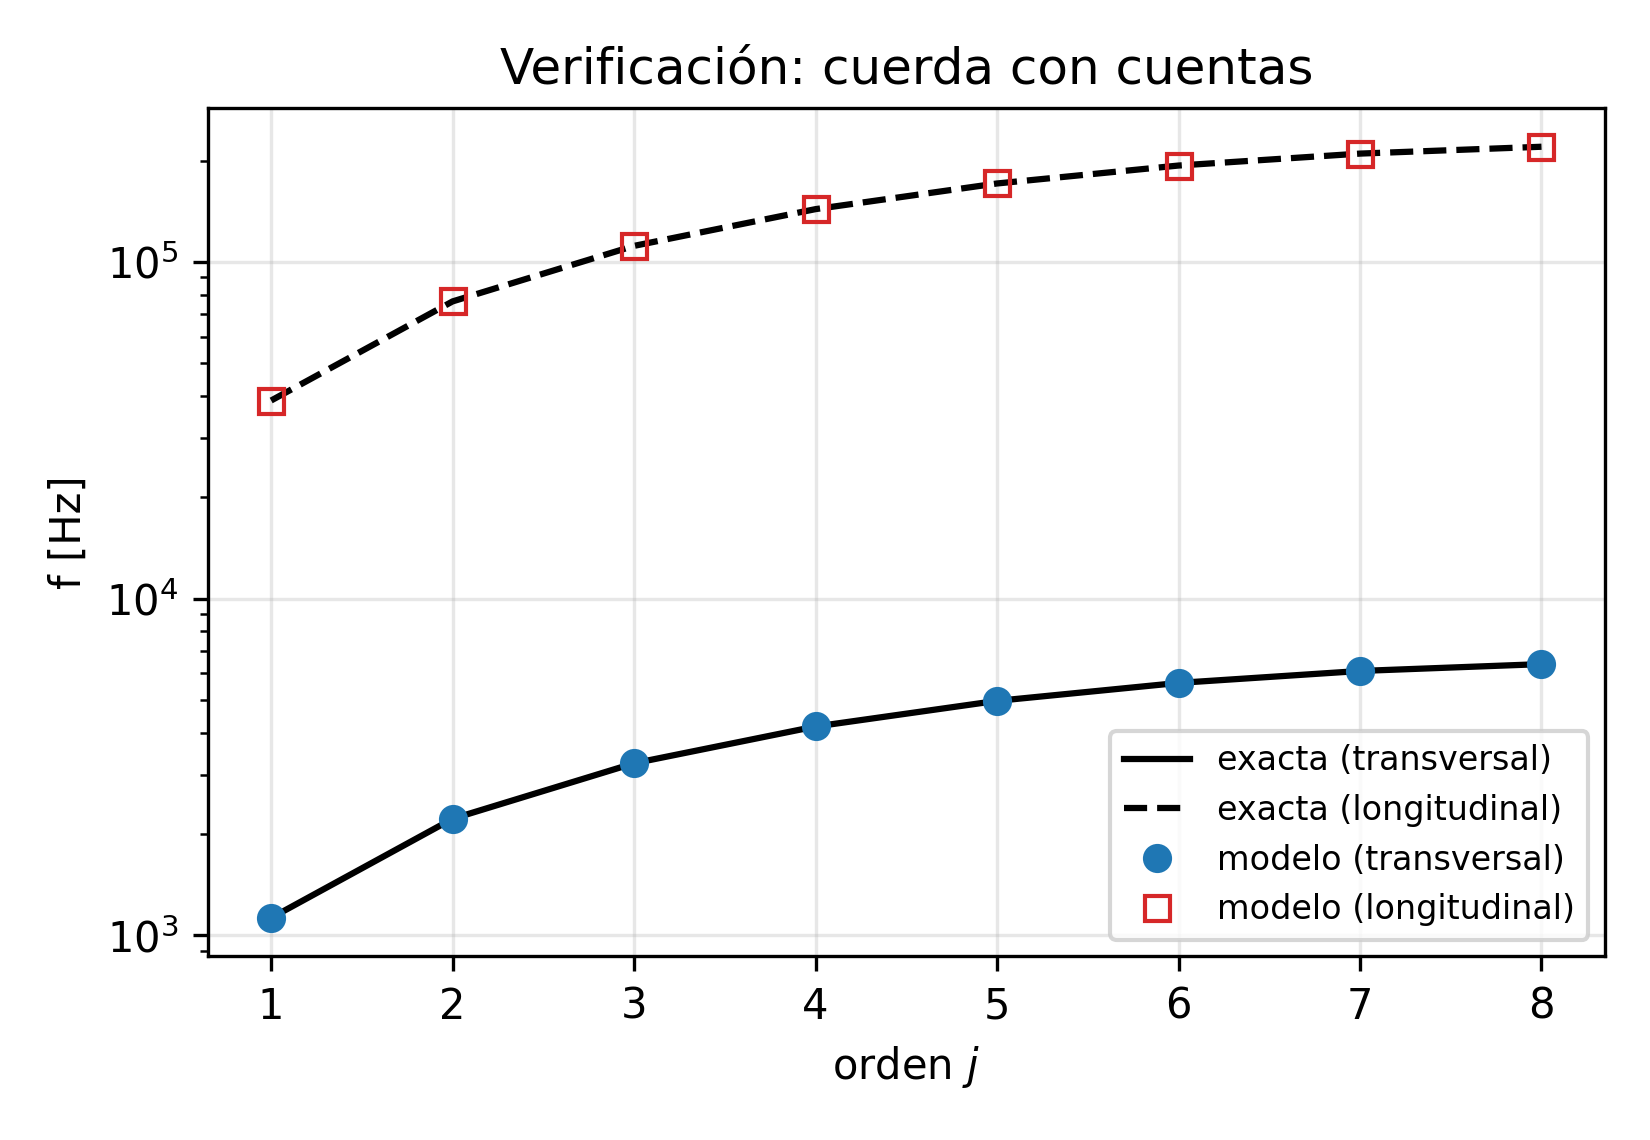
\includegraphics[width=0.55\textwidth]{fig05_benchmark.png}
\caption{Verificación contra la solución exacta de la cuerda con cuentas.}
\label{fig:bench}
\end{figure}

\begin{figure}[H]
\centering
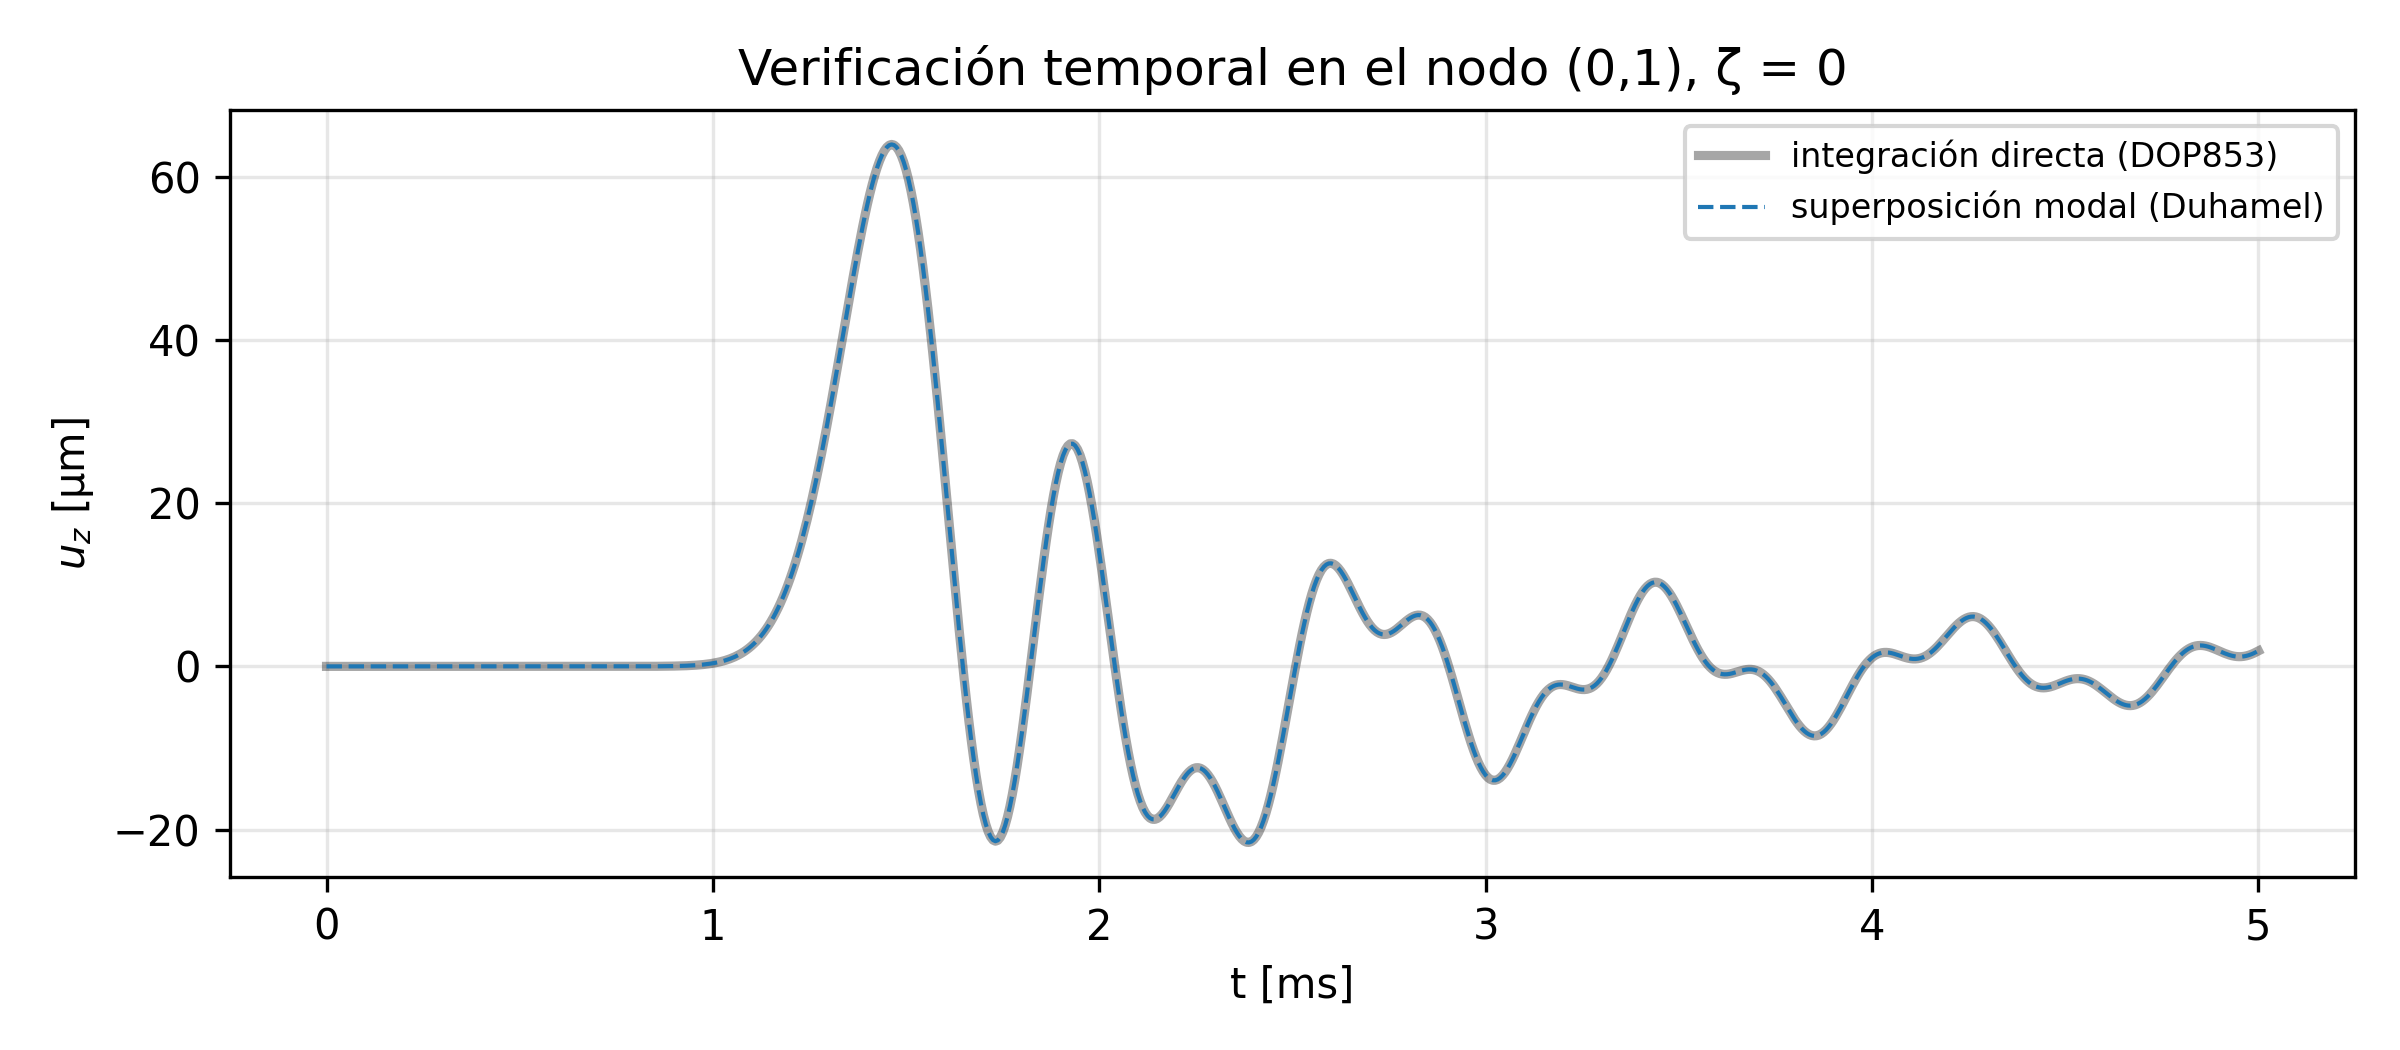
\includegraphics[width=0.85\textwidth]{fig08_verificacion_temporal.png}
\caption{Verificación de la superposición modal contra la integración
numérica directa del subsistema transversal.}
\label{fig:vertemp}
\end{figure}

% =====================================================================
\section{Resultados}\label{sec:resultados}
% =====================================================================

\subsection{Configuración de la red}

\begin{figure}[H]
\centering
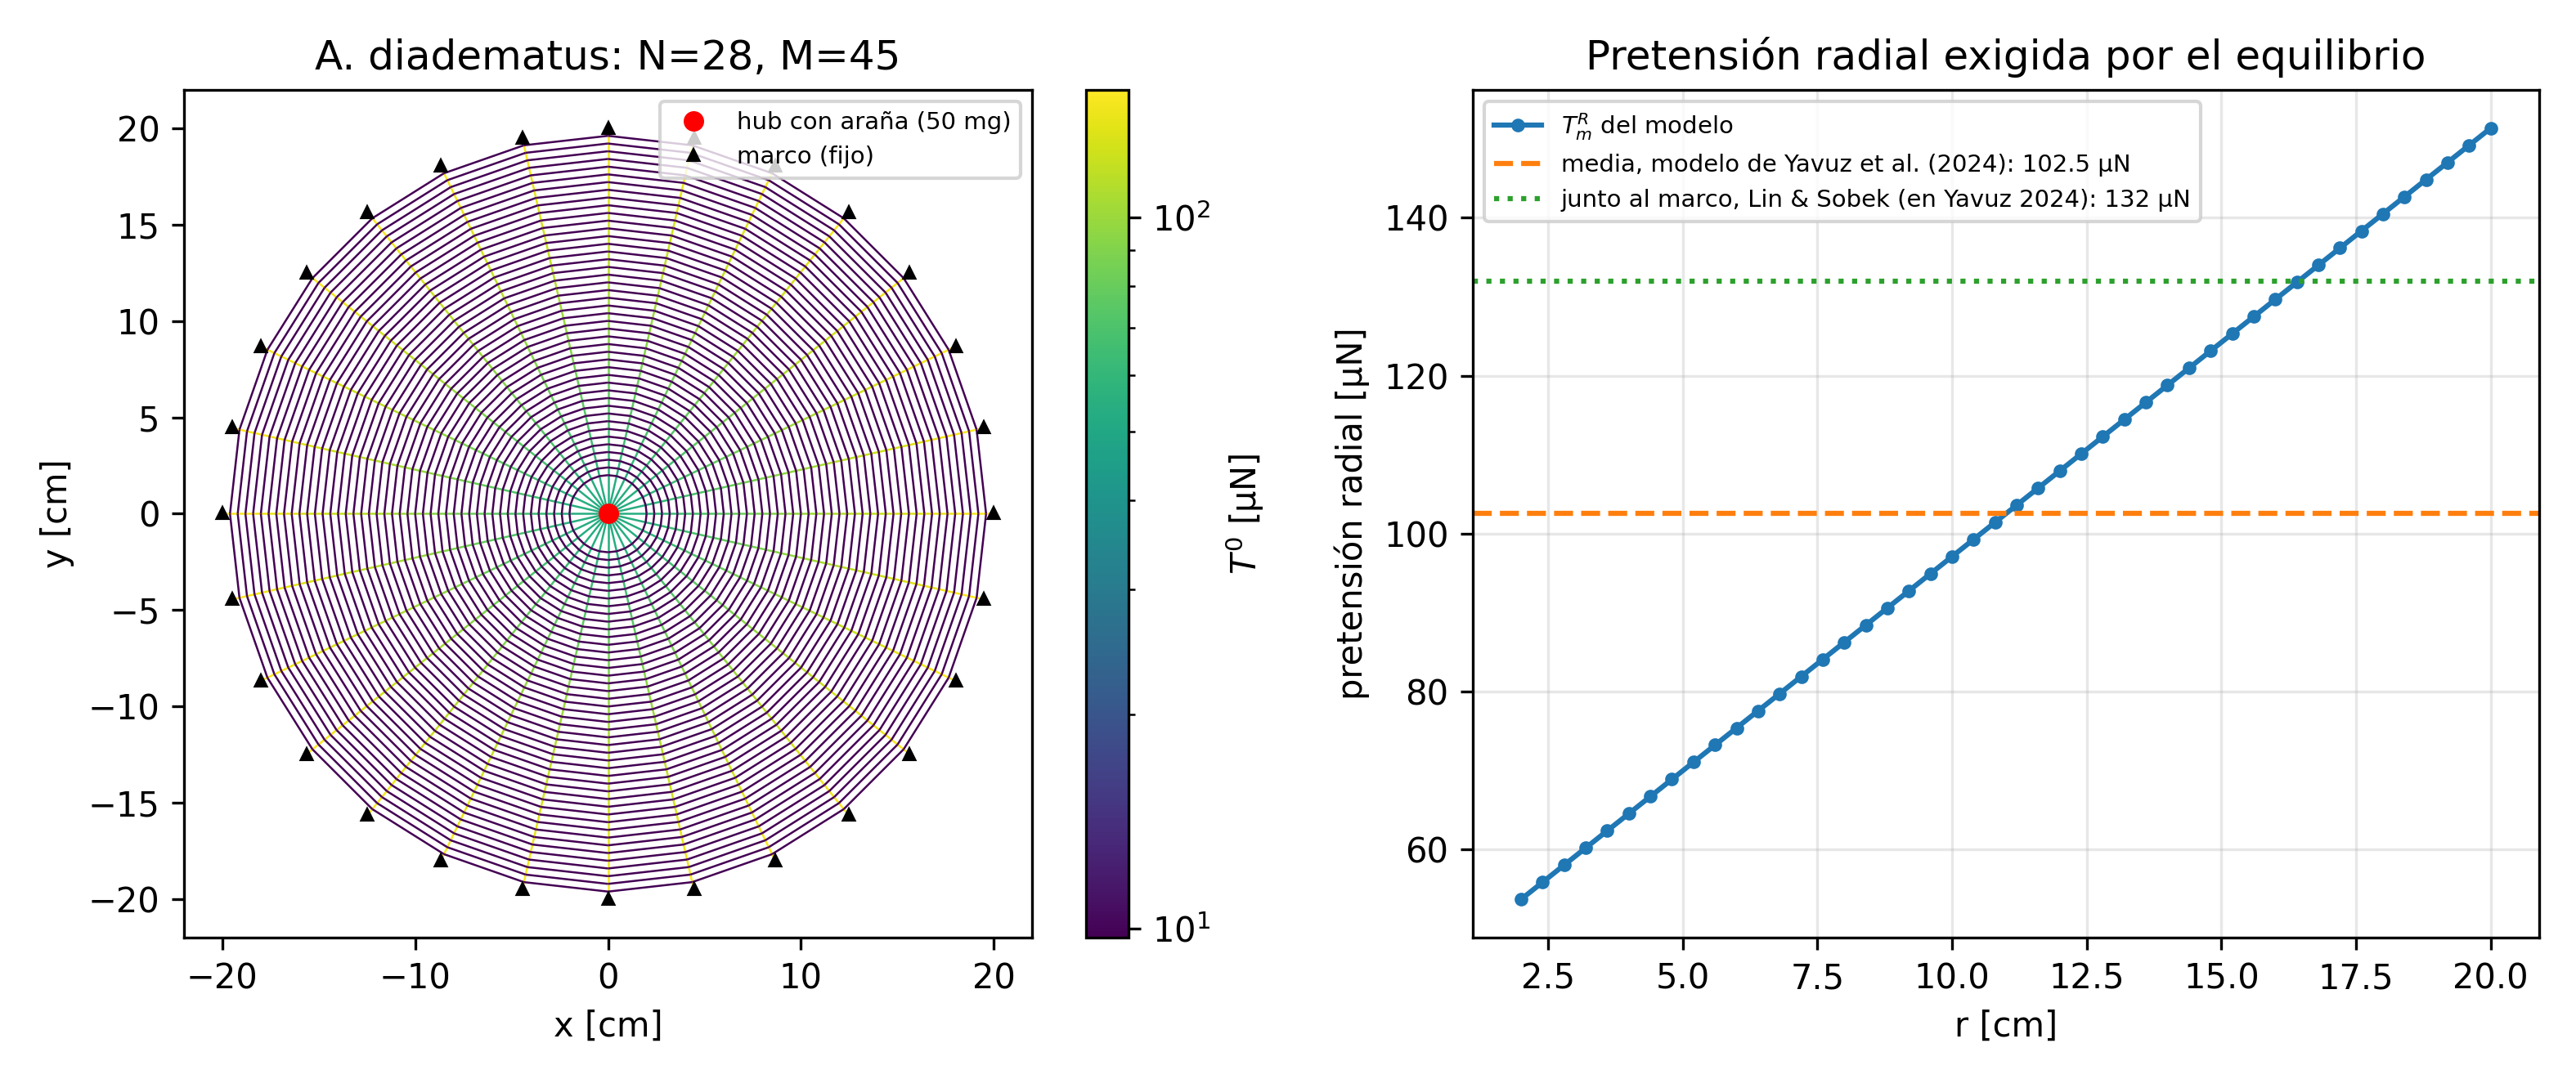
\includegraphics[width=\textwidth]{fig01_geometria.png}
\caption{Izquierda: red modelada, con los hilos coloreados según su
pretensión. Derecha: pretensión radial exigida por el equilibrio
\eqref{eq:recurrencia}, comparada con valores de la literatura.}
\label{fig:geom}
\end{figure}

La figura~\ref{fig:geom} muestra la red de la configuración base. La
pretensión radial crece linealmente de $53.6\uN$ junto al hub a $151.4\uN$
junto al marco. El valor exterior es del mismo orden que los $132\uN$
medidos por Lin y Sobek \cite{linsobek1998}, citados en \cite{yavuz2024}. La
relación entre la pretensión radial media y la masa de la araña es
$\approx 2\uN$/mg, dentro del rango de 1.4 a $7.2\uN$/mg medido por Wirth y
Barth \cite{wirth1992}.

\subsection{Frecuencias naturales y modos de vibración}

La red tiene 1261 modos transversales, con frecuencias entre 2.50 y 3973 Hz,
de los cuales 197 están en la banda de 1 a 1000 Hz. Tiene además 2522 modos
en el plano, entre 65.6 Hz y 169 kHz (figura~\ref{fig:espectro}).

\begin{figure}[H]
\centering
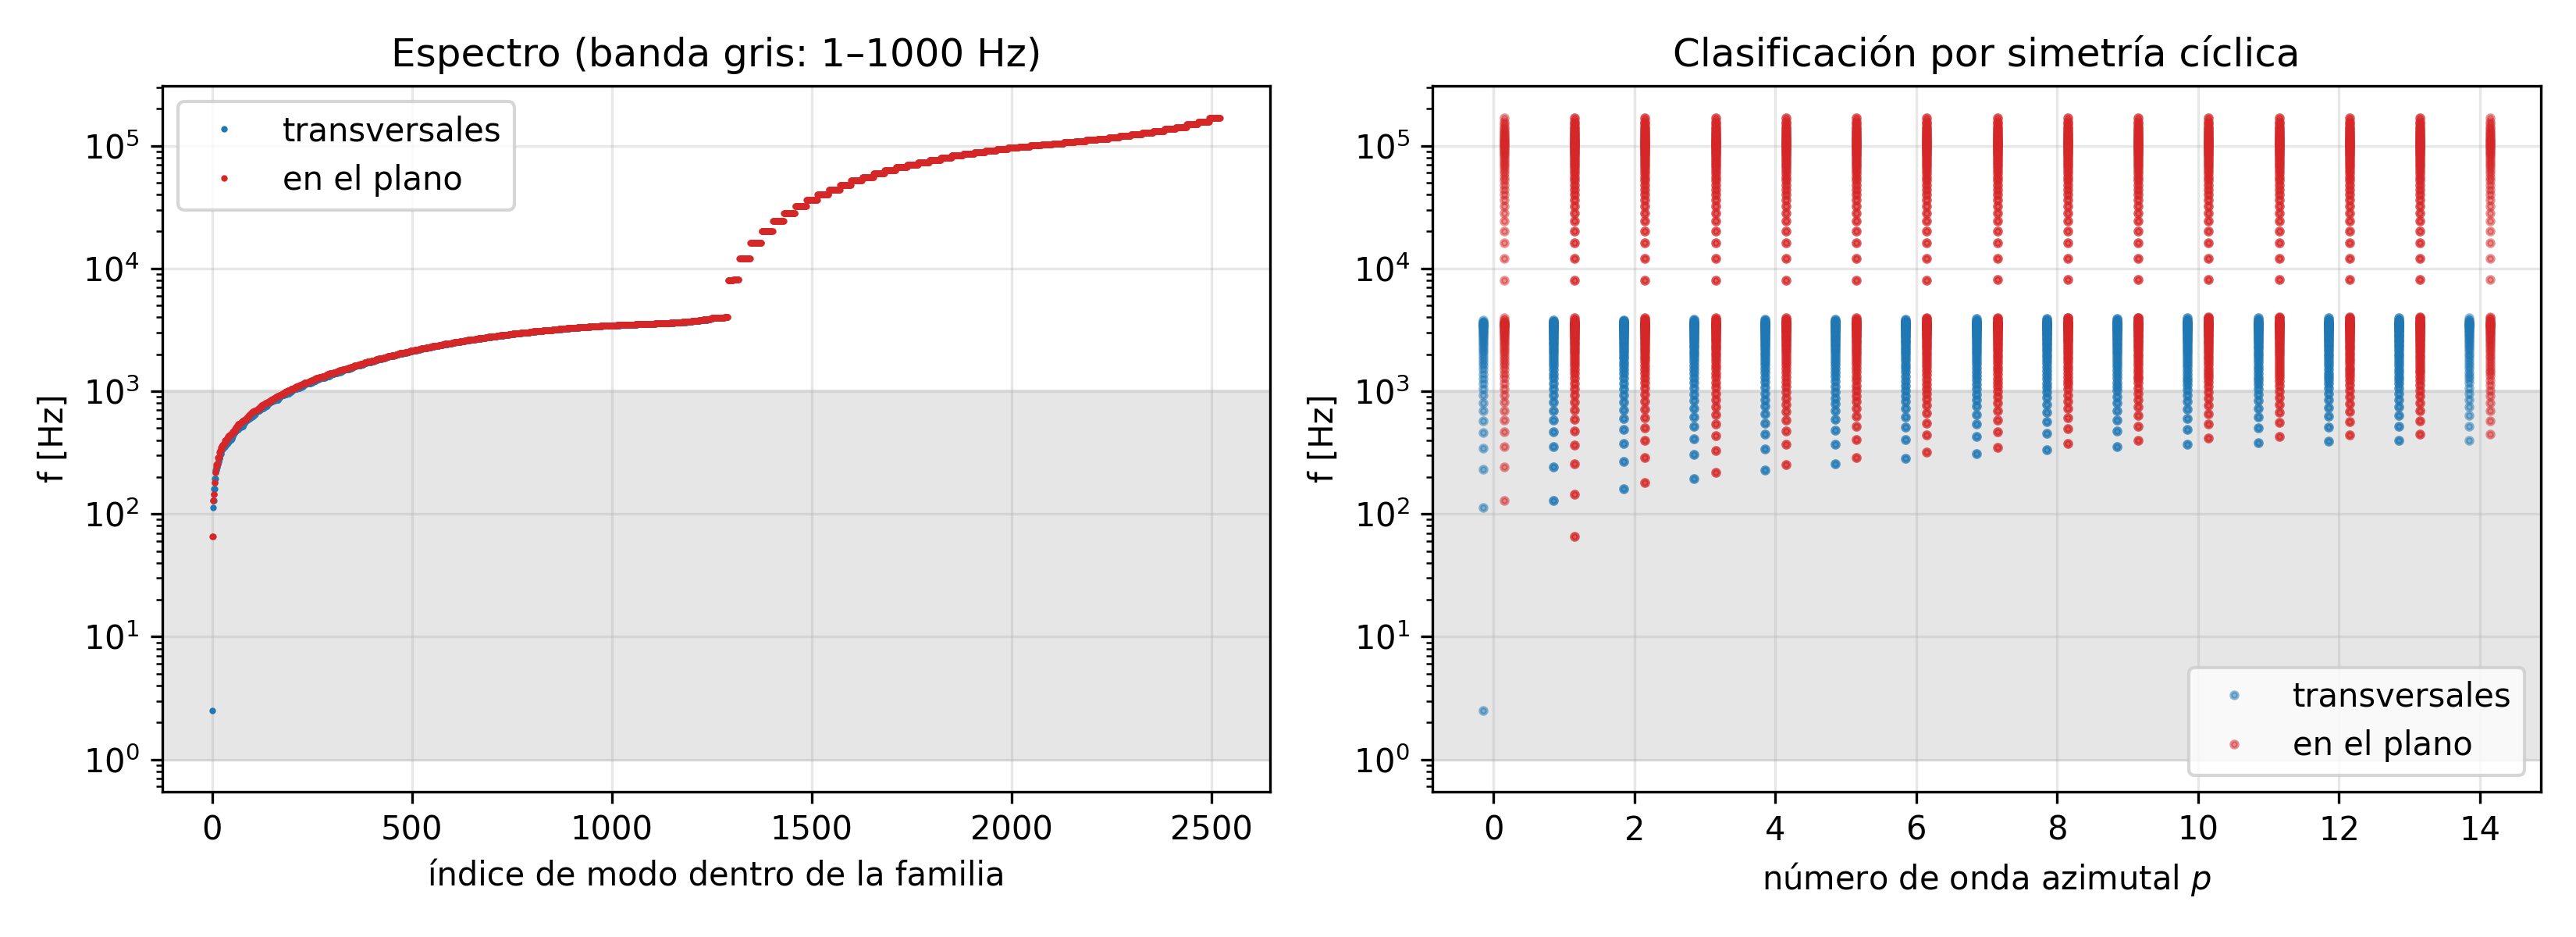
\includegraphics[width=\textwidth]{fig02_espectro.png}
\caption{Izquierda: frecuencias naturales de cada familia, ordenadas de
menor a mayor. Derecha: frecuencia de cada modo frente a su número de onda
azimutal $p$. La franja gris es la banda de 1 a 1000 Hz.}
\label{fig:espectro}
\end{figure}

La figura~\ref{fig:modosT} muestra los seis primeros modos transversales. El
primero (2.50 Hz, $p=0$) es el rebote de la araña: el hub, con sus 50 mg,
sube y baja arrastrando a toda la red. El segundo (112.9 Hz, $p=0$) es el
modo fundamental de la red propiamente dicha: todos los radiales se mueven en
fase, con el hub casi quieto por la inercia de la araña. A partir del
tercero los modos vienen en pares degenerados: 128.0 Hz con $p=1$ y 159.9 Hz
con $p=2$.

\begin{figure}[H]
\centering
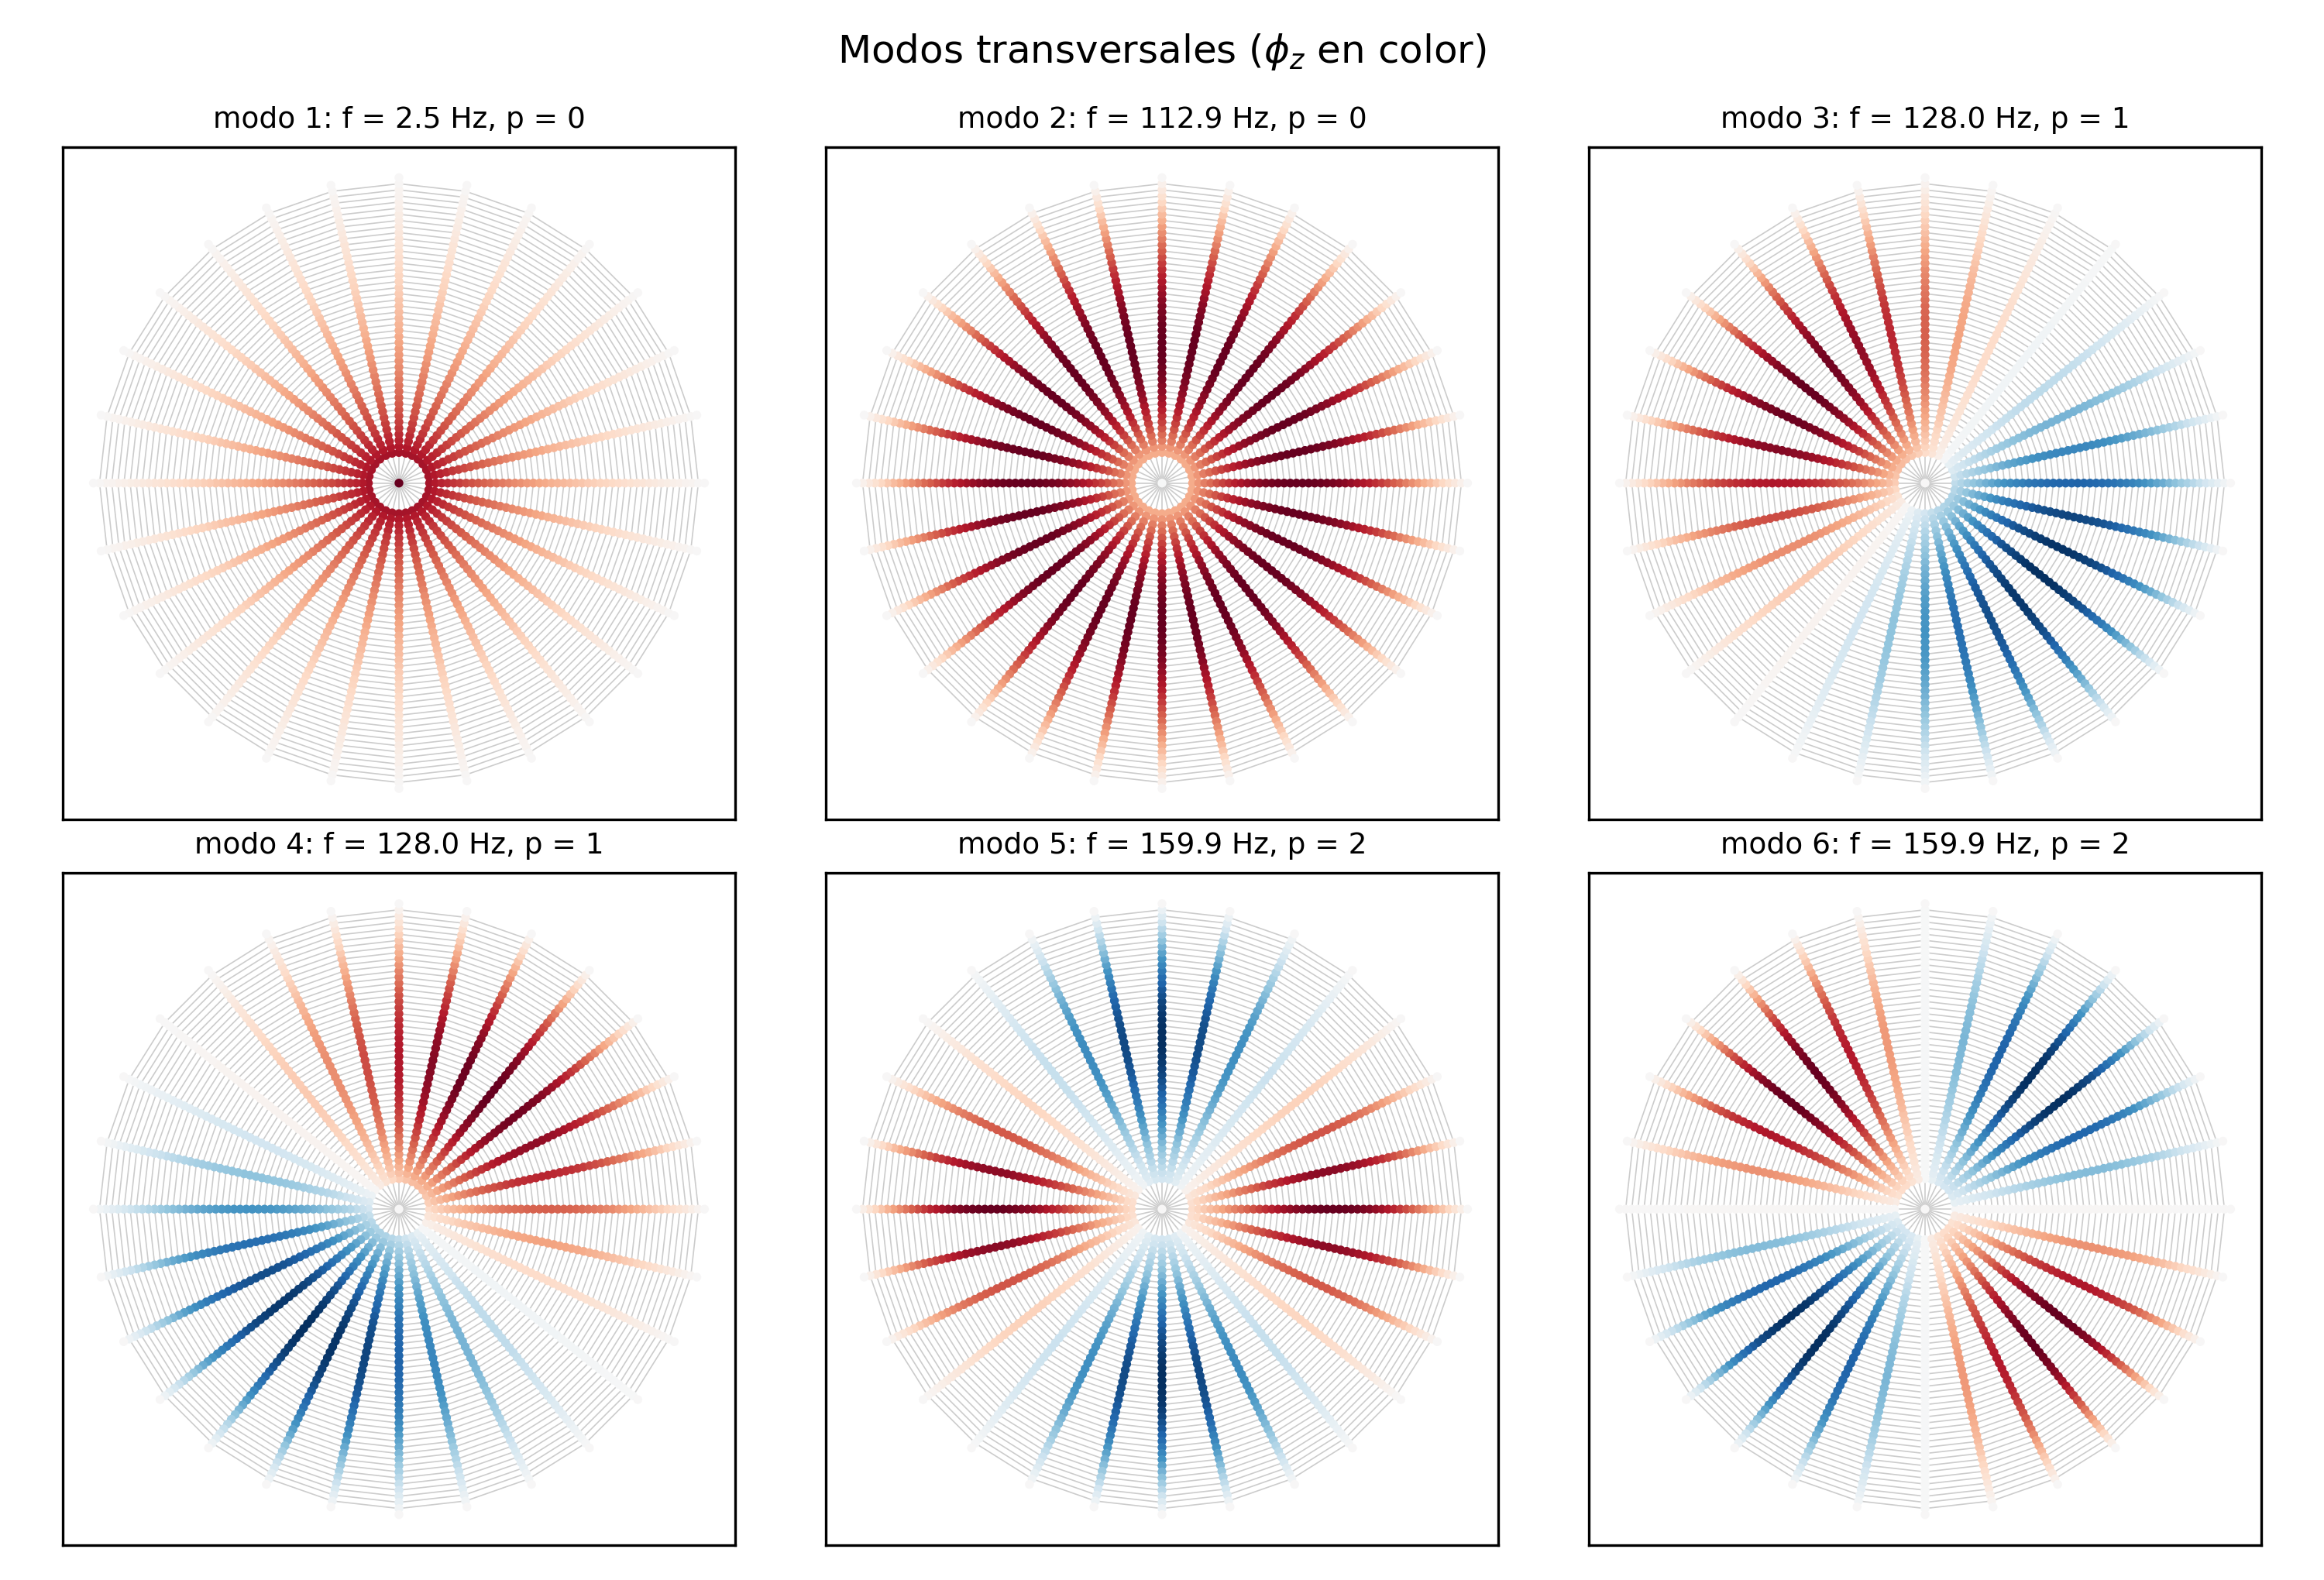
\includegraphics[width=\textwidth]{fig03_modos_transversales.png}
\caption{Primeros seis modos transversales. El color indica el
desplazamiento vertical $\phi_z$ de cada nodo (rojo hacia arriba, azul hacia
abajo).}
\label{fig:modosT}
\end{figure}

En el plano (figura~\ref{fig:modosP}), el primer modo (65.6 Hz, $p=1$) es la
traslación de la araña dentro del plano de la red, y el tercero (128.0 Hz,
$p=0$) es una rotación de la red alrededor del hub.

\begin{figure}[H]
\centering
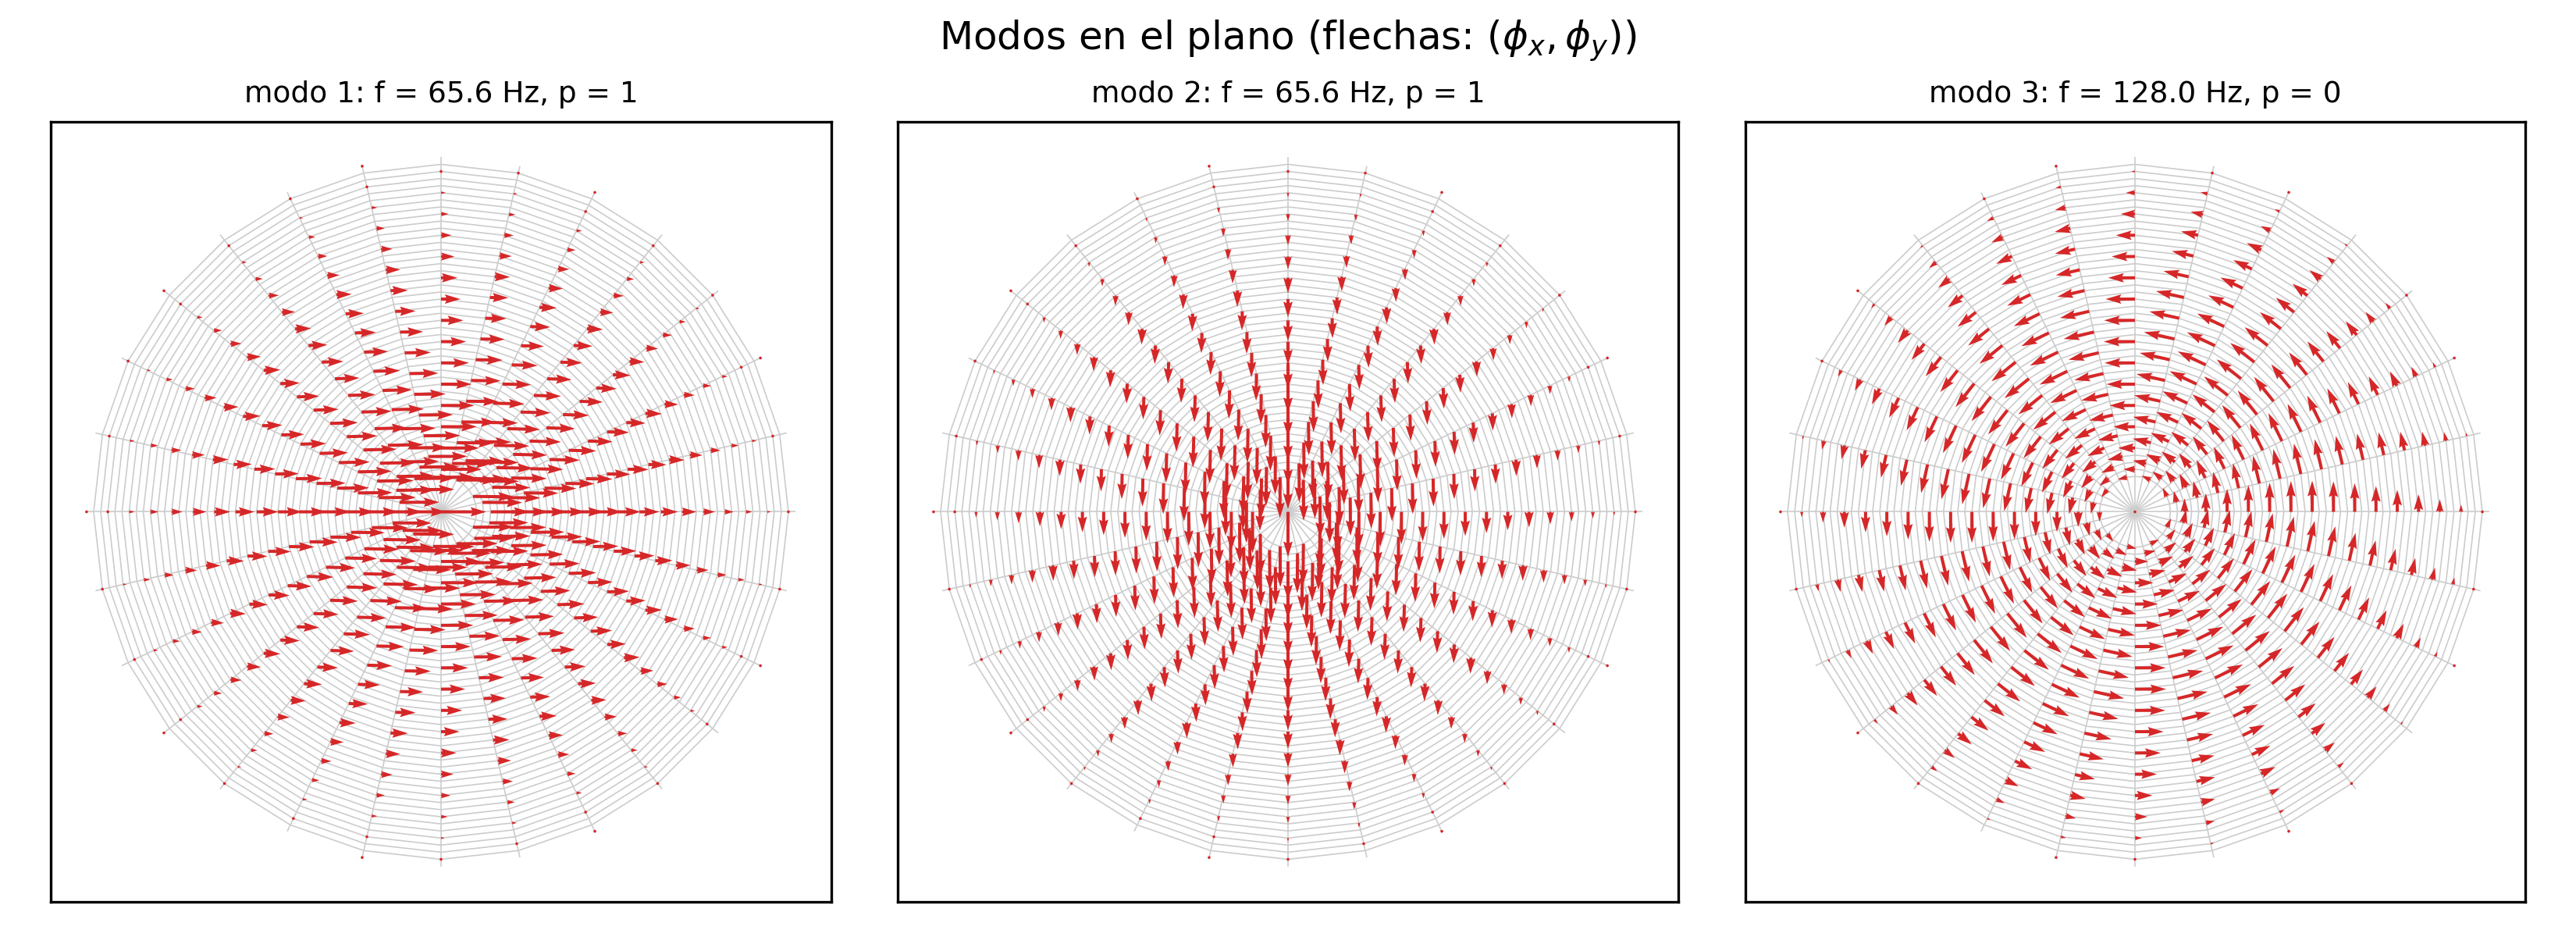
\includegraphics[width=\textwidth]{fig04_modos_plano.png}
\caption{Primeros modos en el plano; las flechas indican el desplazamiento
$(\phi_x,\phi_y)$ de los nodos.}
\label{fig:modosP}
\end{figure}

\subsection{Respuesta a la perturbación de una presa}

La figura~\ref{fig:impulso} muestra el desplazamiento vertical en la presa y
en los observadores tras el impulso. La señal llega primero y con mayor
amplitud al nodo del mismo radial, poco más de 1 ms después del impacto, y
llega más tarde y más débil a los radiales alejados. Después de unos 10 ms la
respuesta queda dominada por oscilaciones lentas de toda la red.

\begin{figure}[H]
\centering
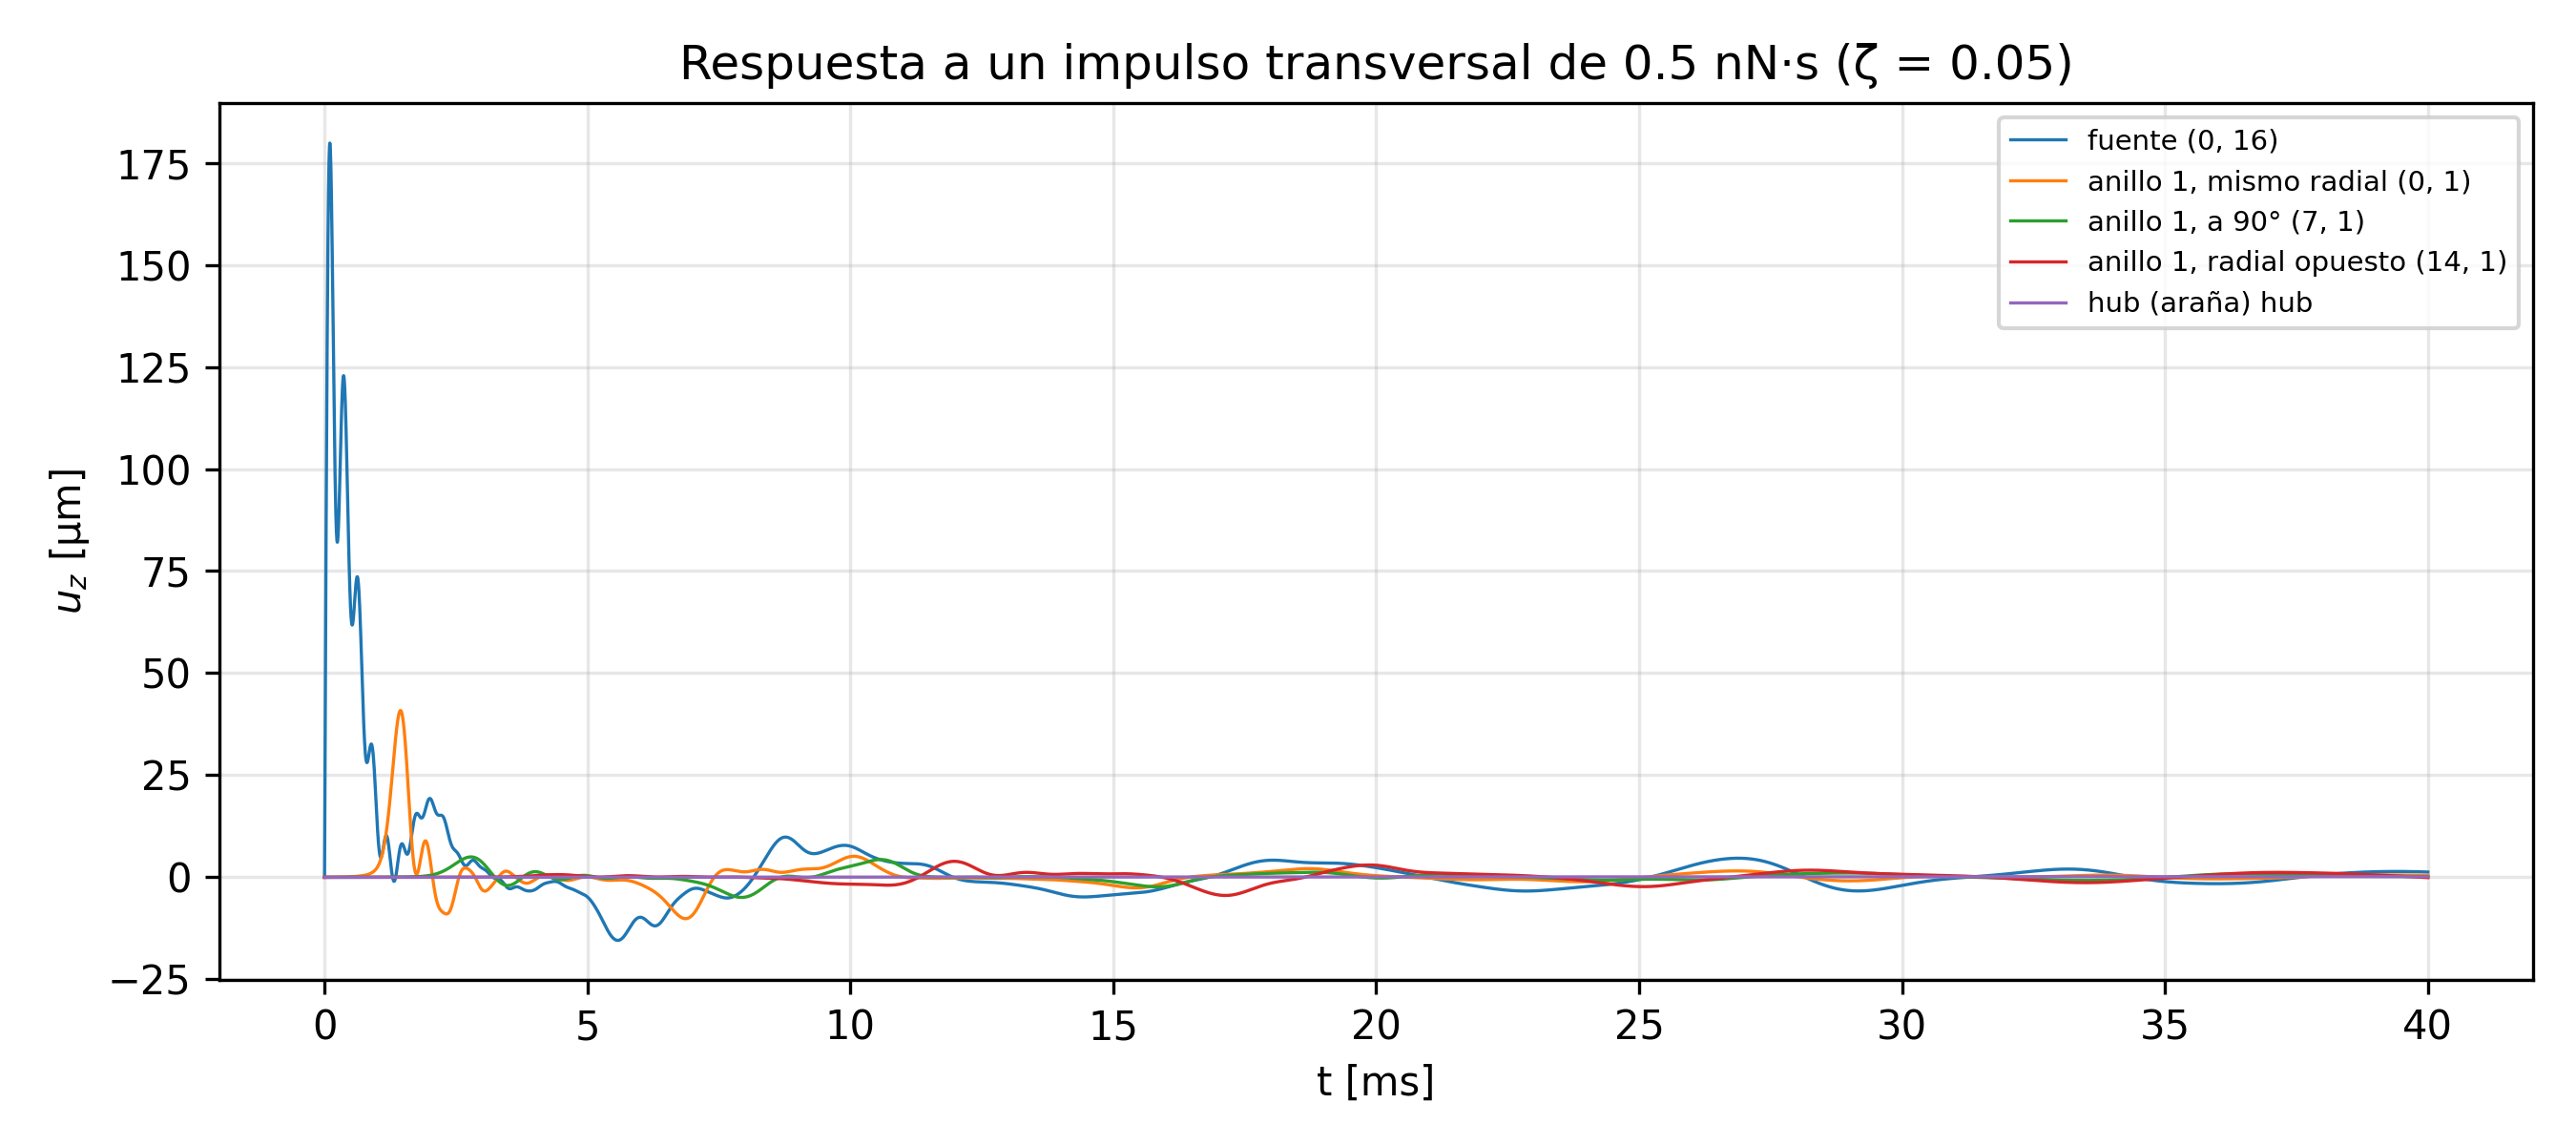
\includegraphics[width=0.9\textwidth]{fig06_respuesta_impulsional.png}
\caption{Desplazamiento vertical $u_z(t)$ en la fuente, en tres observadores
del anillo 1 y en el hub.}
\label{fig:impulso}
\end{figure}

\begin{figure}[H]
\centering
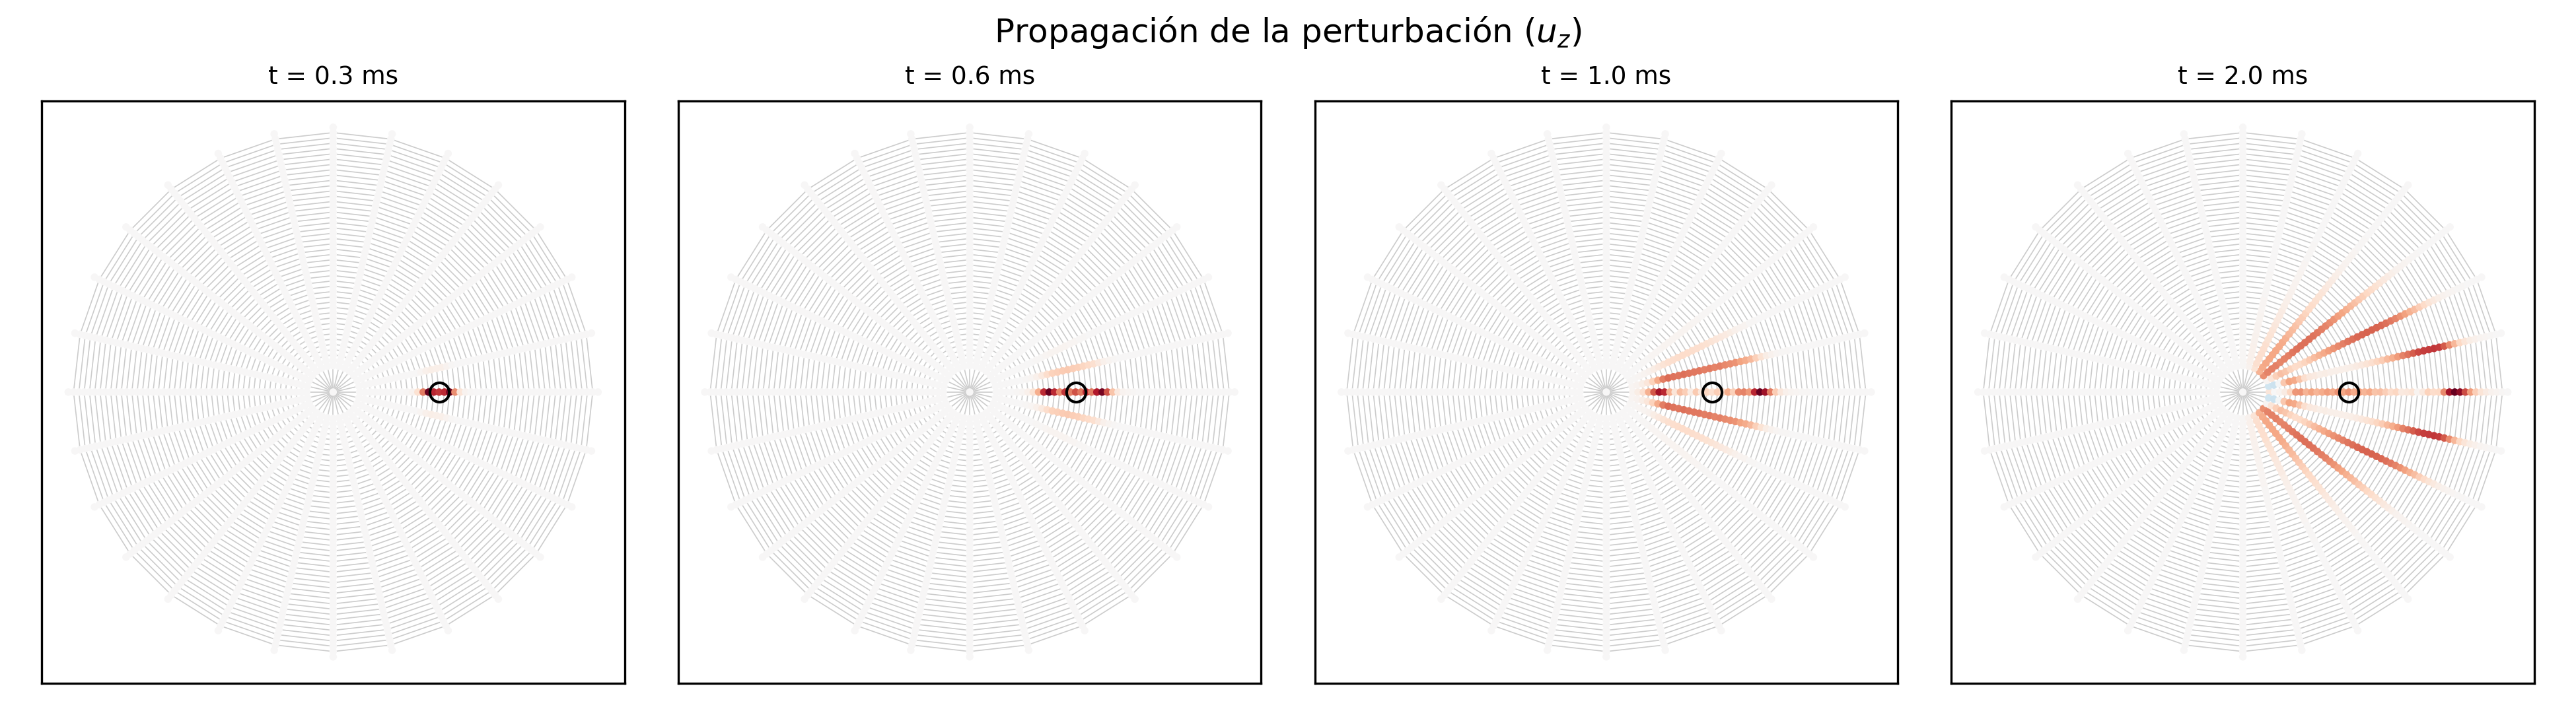
\includegraphics[width=\textwidth]{fig07_instantaneas.png}
\caption{Propagación de la perturbación en cuatro instantes. El círculo
marca la presa.}
\label{fig:snap}
\end{figure}

La figura~\ref{fig:snap} muestra cómo se propaga la perturbación. El frente
viaja principalmente por el radial de la presa y, a medida que avanza, se
reparte hacia los radiales vecinos a través de la espiral. La velocidad
aparente de la onda hacia el hub es de 53 m/s, consistente con la estimación
de cuerda tensa $\sqrt{T^R/\lambda_{\text{ef}}}\approx47$ m/s.

\subsection{Transmisión desde la presa hasta la araña}

La figura~\ref{fig:H} muestra la receptancia entre la presa y cada
observador. Se distinguen tres regiones:
\begin{itemize}
    \item \textbf{Cerca de 2.5 Hz:} todos los observadores tienen el mismo
    pico, porque la red entera se mueve con la araña.
    \item \textbf{Entre 3 y 100 Hz:} la señal depende mucho del observador;
    cada uno tiene una antirresonancia (un mínimo) a una frecuencia distinta
    y las amplitudes difieren hasta en dos órdenes de magnitud.
    \item \textbf{Por encima de 100 Hz:} aparecen las resonancias de la red y
    las curvas se vuelven a acercar.
\end{itemize}

\begin{figure}[H]
\centering
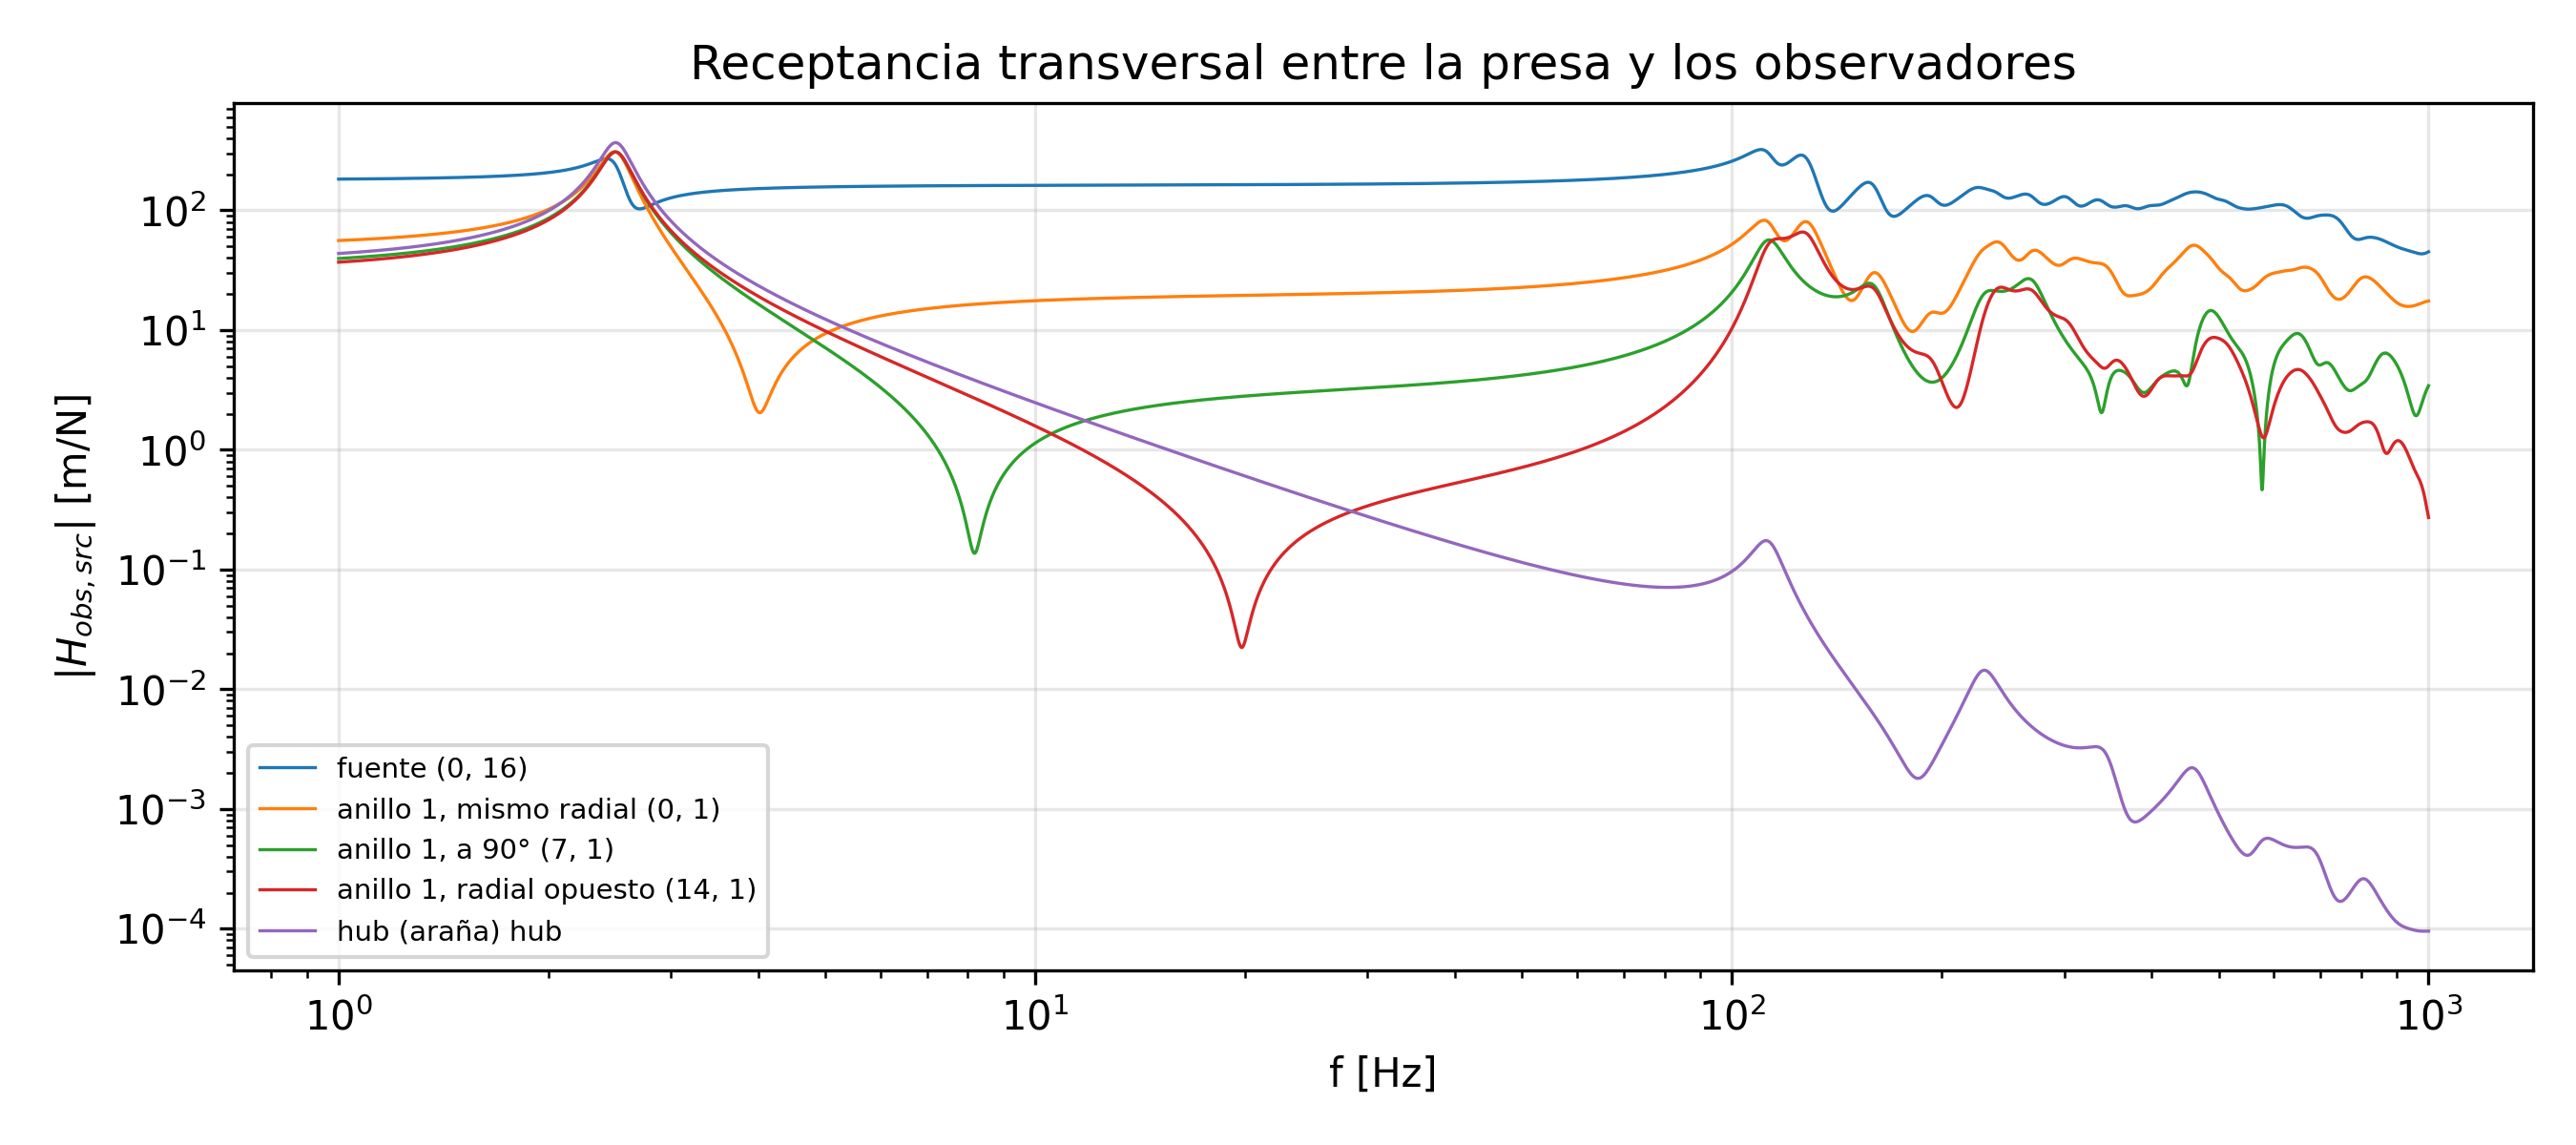
\includegraphics[width=0.9\textwidth]{fig09_transferencia.png}
\caption{Módulo de la receptancia $|H_{obs,src}(\omega)|$ entre la presa y
los observadores.}
\label{fig:H}
\end{figure}

\begin{figure}[H]
\centering
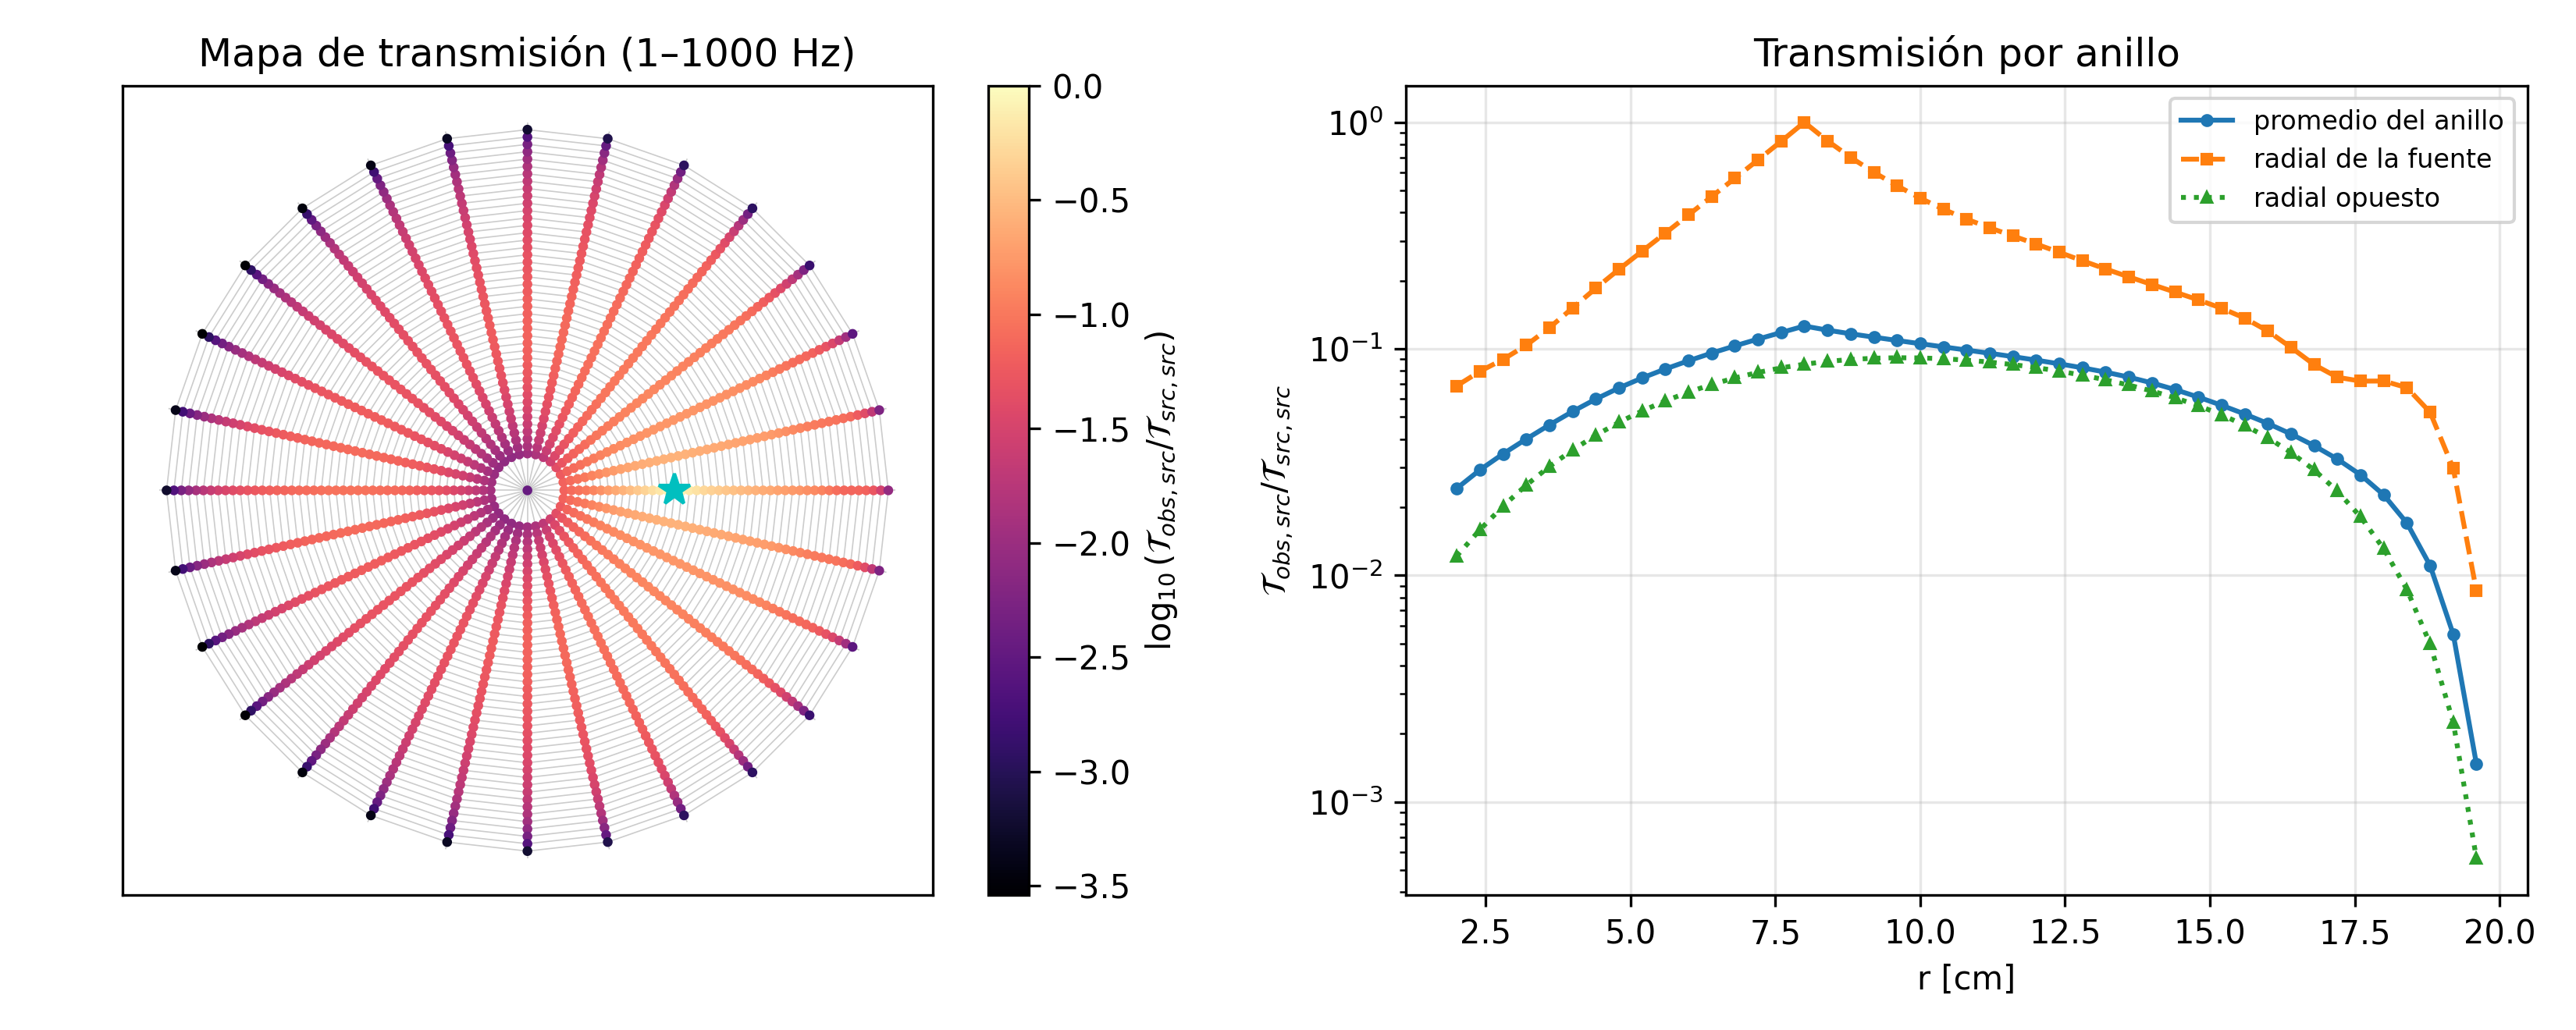
\includegraphics[width=\textwidth]{fig10_mapa_transmision.png}
\caption{Índice de transmisión normalizado
$\mathcal{T}_{obs,src}/\mathcal{T}_{src,src}$ en la banda de 1 a 1000 Hz,
para todos los nodos (izquierda) y por anillo (derecha).}
\label{fig:mapa}
\end{figure}

El mapa de la figura~\ref{fig:mapa} muestra que la señal se concentra en el
radial de la presa y en sus vecinos, y decae hacia el hub y hacia el marco.
La tabla~\ref{tab:T} y la figura~\ref{fig:bandas} comparan el índice en las
dos bandas.

\begin{table}[H]
\centering\small
\caption{Índice de transmisión normalizado $\mathcal{T}_{obs,src}/\mathcal{T}_{src,src}$
desde la presa (nodo $(0,16)$).}
\label{tab:T}
\begin{tabular}{@{}lcc@{}}
\toprule
Observador & 1--1000 Hz & 5--30 Hz \\
\midrule
Anillo 1, mismo radial $(0,1)$ & $6.86\times10^{-2}$ & $1.31\times10^{-2}$ \\
Anillo 1, a $90^\circ$ $(7,1)$ & $1.09\times10^{-2}$ & $2.69\times10^{-4}$ \\
Anillo 1, radial opuesto $(14,1)$ & $1.22\times10^{-2}$ & $1.66\times10^{-4}$ \\
Hub (araña) & $3.49\times10^{-3}$ & $3.01\times10^{-4}$ \\
\bottomrule
\end{tabular}
\end{table}

\begin{figure}[H]
\centering
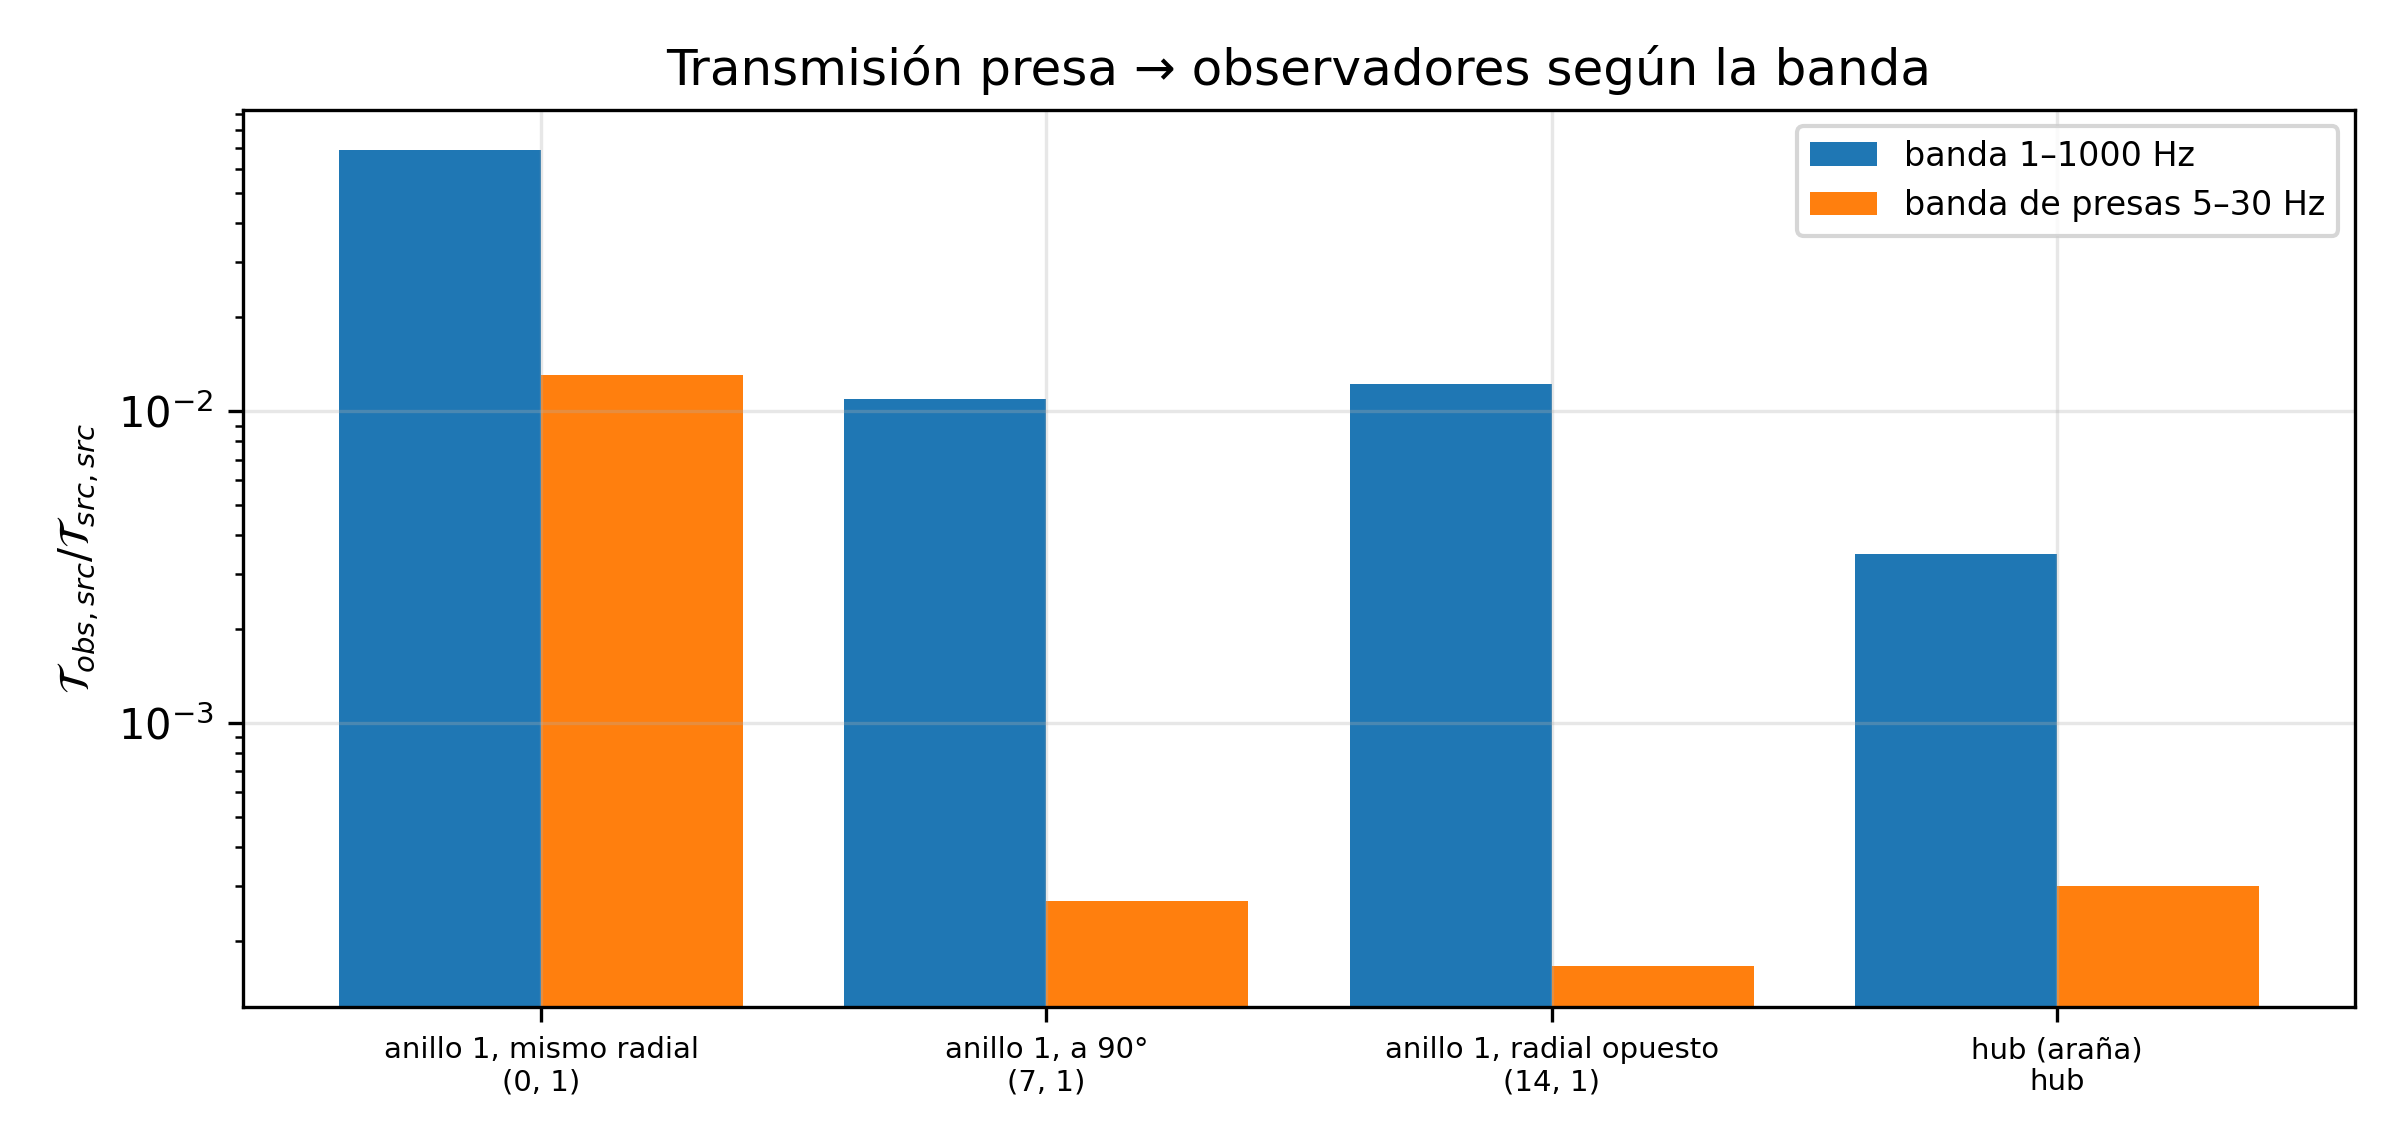
\includegraphics[width=0.8\textwidth]{fig12_transmision_bandas.png}
\caption{Índice normalizado para los observadores en las dos bandas.}
\label{fig:bandas}
\end{figure}

En la banda de 1 a 1000 Hz, el mismo radial recibe unas 6 veces más señal
que los radiales a $90^\circ$ o el opuesto. En la banda de presas, esa
diferencia sube a un factor de 50 a 80, es decir, 17 a 19 dB. A lo largo del
radial de la presa, la señal en esa banda cae unos 19 dB en los 6 cm que
separan la presa del anillo 1.

\subsection{Sensibilidad al amortiguamiento}

La figura~\ref{fig:zeta} muestra que el índice disminuye al aumentar $\zeta$
y tiende a crecer como $1/\zeta$ cuando el amortiguamiento es pequeño, como
predice el análisis de la sección~\ref{sec:modelo}. Por esta razón los
valores absolutos del índice dependen de $\zeta$, pero los valores
normalizados, que comparan observadores con el mismo $\zeta$, son más
robustos.

\begin{figure}[H]
\centering
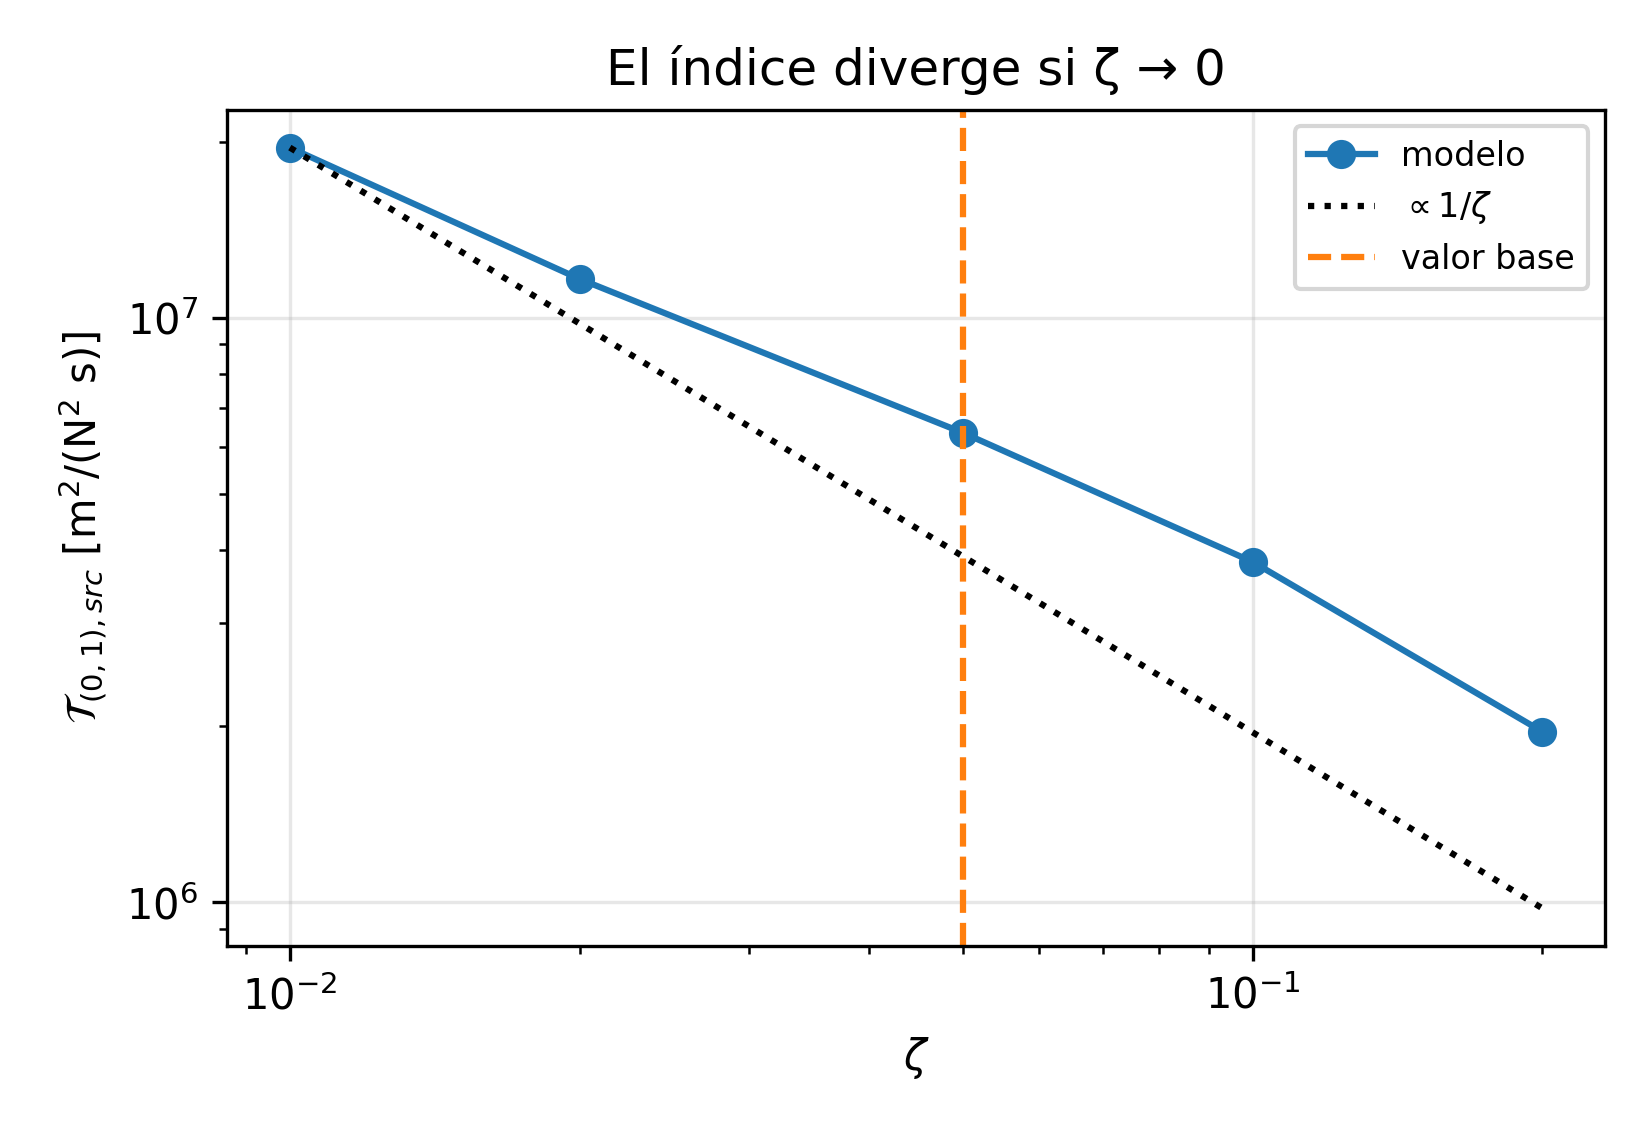
\includegraphics[width=0.55\textwidth]{fig11_sensibilidad_zeta.png}
\caption{Índice de transmisión hacia el nodo $(0,1)$ en función del
amortiguamiento.}
\label{fig:zeta}
\end{figure}

\subsection{Efecto de la araña en el centro}

\begin{table}[H]
\centering\small
\caption{Comparación entre una red con centro fijo y una con hub libre que
lleva la masa de la araña.}
\label{tab:hub}
\begin{tabular}{@{}lcc@{}}
\toprule
 & Centro fijo & Hub libre, $m_a=50$ mg \\
\midrule
Primera frecuencia transversal & 112.8 Hz & 2.50 Hz \\
Modos transversales en 1--1000 Hz & 196 & 197 \\
$\mathcal{T}/\mathcal{T}_{src}$ mismo radial (1--1000 / 5--30 Hz) & $6.6\times10^{-2}$ / $1.5\times10^{-2}$ & $6.9\times10^{-2}$ / $1.3\times10^{-2}$ \\
$\mathcal{T}/\mathcal{T}_{src}$ a $90^\circ$ (1--1000 / 5--30 Hz) & $8.6\times10^{-3}$ / $4.1\times10^{-4}$ & $1.1\times10^{-2}$ / $2.7\times10^{-4}$ \\
$\mathcal{T}/\mathcal{T}_{src}$ radial opuesto (1--1000 / 5--30 Hz) & $9.8\times10^{-3}$ / $1.0\times10^{-5}$ & $1.2\times10^{-2}$ / $1.7\times10^{-4}$ \\
\bottomrule
\end{tabular}
\end{table}

Con la araña en un hub libre, la primera frecuencia transversal baja de
112.8 a 2.50 Hz, un factor de 45. En la banda de presas, la señal que llega
al radial opuesto aumenta unas 17 veces, mientras que la del radial de la
presa casi no cambia (tabla~\ref{tab:hub}).

% =====================================================================
\section{Discusión}\label{sec:discusion}
% =====================================================================

\paragraph{La tensión controla la vibración transversal.} La separación
exacta \eqref{eq:desacople} muestra que las vibraciones perpendiculares a la
red dependen solo de la relación $T^0/L^0$ y de las masas, y no del módulo de
Young de la seda. Esto significa que, para las vibraciones transversales,
las variables que la araña puede ajustar al construir la red (la tensión de
los hilos y su espaciado) son exactamente las que determinan la respuesta.
Este resultado es consistente con la observación de que las arañas modifican
la tensión de los radiales para cambiar su capacidad de detectar presas en
distintos sectores de la red \cite{nakata2010}.

\paragraph{La araña cambia el espectro de la red.} La masa de la araña es
unas 190 veces mayor que la de la seda: con los parámetros de la
tabla~\ref{tab:param}, toda la red pesa unos 0.26 mg, frente a los 50 mg de
la araña. Por eso aparece un modo de 2.5 Hz en el que
la araña rebota sobre la red y, en los demás modos, el hub se comporta casi
como un punto fijo. Aun así, el hub libre permite que parte de la señal pase
de un radial a otro a través del centro, lo que explica el aumento de la
transmisión hacia el radial opuesto en la tabla~\ref{tab:hub}. Esto indica
que un modelo con el centro fijo subestima el acople entre radiales.

\paragraph{La información sobre la dirección está en una banda de
frecuencias.} El contraste entre el radial de la presa y los demás es pequeño
cuando se integra en toda la banda de 1 a 1000 Hz, pero es grande en la
banda de 5 a 30 Hz. La razón es que fuera de esa banda la respuesta está
dominada por modos que mueven toda la red (el rebote de la araña a 2.5 Hz y
los modos de la red por encima de 100 Hz), mientras que entre ellos la señal
viaja sobre todo por el radial de la presa. Coincide con que la banda de 5 a
30 Hz es justamente donde vibran las presas atrapadas \cite{landolfa1996}.
Mortimer et al.\ \cite{mortimer2019decoding} encontraron, con un modelo de
elementos finitos de la misma especie, que comparar la amplitud de la
vibración entre las ocho patas en el centro basta para determinar la
dirección de la presa. Los resultados de este modelo apuntan en el mismo
sentido: con una diferencia de 17 a 19 dB entre radiales, las patas de la
araña recibirían señales claramente distintas según la dirección de la
presa.

\paragraph{Comparación con medidas.} La atenuación de unos 19 dB en 6 cm a
lo largo del radial es del mismo orden que la de 22 dB en unos 12 cm medida
por Landolfa y Barth \cite{landolfa1996} para ondas transversales. La
comparación es solo orientativa, porque ellos estudiaron \textit{Nephila
clavipes} y usaron otra métrica, pero indica que el modelo produce
atenuaciones de una magnitud realista. Lo mismo ocurre con la pretensión
junto al marco (151 frente a $132\uN$) y con la relación entre la tensión y
la masa de la araña.

\paragraph{Limitaciones.} Hasta ahora solo se ha analizado la transmisión
de vibraciones transversales. Mortimer et al.\ \cite{mortimer2019decoding}
encontraron que las ondas en el plano (longitudinales) aportan información
sobre la dirección de la presa, por lo que el análisis de la familia en el
plano será necesario en el ciclo 3. Además, el modelo supone una red
circular, horizontal y simétrica, con el marco rígido; no incluye la masa
del pegamento de la espiral, y usa para la seda viscosa un módulo que no es
válido a la deformación real de la espiral. Estas limitaciones se discuten
en la sección~\ref{sec:dificultades}.

% =====================================================================
\section{Conclusiones parciales}\label{sec:conclusiones}
% =====================================================================

\begin{enumerate}
    \item Se construyó un modelo lagrangiano de la telaraña orbicular que
    incluye la rigidez elástica y la geométrica de los hilos. Para que el
    modelo sea consistente, la red debe estar anclada a un marco y las
    pretensiones deben cumplir la condición de equilibrio
    \eqref{eq:recurrencia}, según la cual la tensión radial crece del centro
    hacia afuera.
    \item El movimiento en el plano y el transversal están exactamente
    desacoplados. Las vibraciones transversales dependen solo de las
    pretensiones, las longitudes y las masas, que son las variables que la
    araña controla al construir la red.
    \item La implementación numérica se verificó contra una solución exacta,
    contra integración directa y contra la simetría del sistema, con errores
    menores a $10^{-9}$. La herramienta está lista para comparar geometrías.
    \item Para \textit{A.~diadematus}, la red tiene un modo de rebote de la
    araña a 2.5 Hz y su modo fundamental a 113 Hz. Los demás modos se
    organizan en pares degenerados según su número de onda azimutal.
    \item La información sobre la dirección de la presa se concentra en la
    banda de 5 a 30 Hz, donde el radial de la presa recibe entre 50 y 80
    veces más señal que los demás. Por tanto, las comparaciones entre
    geometrías del ciclo 3 deben hacerse en esa banda y no con un índice de
    banda ancha.
    \item Modelar el hub libre con la masa de la araña cambia de forma
    importante el espectro y aumenta el acople entre radiales, por lo que
    este será el modelo principal del ciclo 3.
\end{enumerate}

% =====================================================================
\section{Estado de avance}\label{sec:avance}
% =====================================================================

\subsection{Actividades realizadas y ajustes al modelo}

En el ciclo 2 se cumplieron las actividades de las semanas 7 a 12 del
cronograma: implementación numérica y verificación de $\mathbf{M}$ y
$\mathbf{K}$ (semana 7), solución del problema de valores propios (semana 8),
clasificación de modos por familia (semana 9), respuesta temporal ante una
perturbación impulsional (semana 10) y cálculo de la receptancia y del
índice de transmisión para la configuración base (semana 11).

Durante la implementación fue necesario ajustar el modelo del anteproyecto
en cinco puntos:
\begin{itemize}
    \item Se reemplazó el borde exterior libre por un borde anclado al marco
    y se impuso la condición de equilibrio de las pretensiones
    (sección~\ref{sec:equilibrio}). Con el borde libre, la fuerza neta sobre
    los nodos exteriores era de $2.82\,T^R_1$, es decir, la configuración no
    estaba en equilibrio.
    \item Se demostró que la separación entre familias de modos es exacta, y
    no aproximada como se había planteado.
    \item Se incluyó amortiguamiento modal, sin el cual el índice de
    transmisión diverge.
    \item Se corrigió la notación de la función de transferencia, que en el
    anteproyecto multiplicaba un vector de tres componentes por una matriz de
    dimensión $3NM$.
    \item Se reemplazó el centro fijo por un hub libre con la masa de la
    araña, siguiendo a \cite{yavuz2024}.
\end{itemize}

\subsection{Porcentaje de avance}\label{sec:porcentaje}

\begin{table}[H]
\centering\small
\caption{Avance por ciclo, ponderado por semanas del cronograma.}
\begin{tabular}{@{}lccc@{}}
\toprule
Ciclo & Peso & Avance del ciclo & Aporte \\
\midrule
Ciclo 1 --- Definición y modelado (sem.\ 1--6) & 33.3\,\% & 100\,\% & 33.3\,\% \\
Ciclo 2 --- Caracterización (sem.\ 7--12) & 33.3\,\% & 100\,\% & 33.3\,\% \\
Ciclo 3 --- Simulación comparativa (sem.\ 13--16) & 22.2\,\% & 0\,\% & 0\,\% \\
Cierre (sem.\ 17--18) & 11.1\,\% & 0\,\% & 0\,\% \\
\midrule
\textbf{Total} & 100\,\% & & \textbf{66.7\,\%} \\
\bottomrule
\end{tabular}
\end{table}

\subsection{Dificultades y retos pendientes}\label{sec:dificultades}

\begin{itemize}
    \item \textbf{Elección de la métrica de transmisión.} El índice
    integrado en una banda ancha queda dominado por los modos globales y
    pierde la información direccional (tabla~\ref{tab:T}). Se requiere
    comparar geometrías tanto en la banda de presas como con una métrica
    temporal, como la amplitud o el tiempo de primera llegada.
    \item \textbf{Linealidad de la espiral.} La pretensión espiral de
    $9.7\uN$ corresponde a una deformación de $\approx71\,\%$ si se usa el
    módulo inicial de 3 MPa, lo cual está fuera del régimen lineal de la
    seda viscosa. Esto solo afecta a los modos en el plano, porque la
    familia transversal no depende de $\kappa$; para los modos en el plano
    se debe usar un módulo tangente. En los radiales la deformación de
    pretensión es de $0.085\,\%$ y el modelo lineal es adecuado.
    \item \textbf{Masa del pegamento.} No se encontró un valor de masa por
    unidad de longitud de las gotas de la espiral de captura; por ahora
    solo se incluye la fibra. Esa masa adicional reduciría las frecuencias
    y la velocidad de onda.
    \item \textbf{Amortiguamiento.} $\zeta=0.05$ proviene de ensayos de
    histéresis cuasiestáticos; el amortiguamiento a pequeña amplitud y la
    resistencia aerodinámica pueden ser distintos. Por eso las comparaciones
    entre geometrías se harán con índices normalizados y con análisis de
    sensibilidad (figura~\ref{fig:zeta}).
    \item \textbf{Simplificaciones geométricas.} La red es circular,
    simétrica y horizontal (sin peso), y el marco es rígido. Las redes
    reales son verticales y asimétricas, y el peso de la araña redistribuye
    las pretensiones \cite{yavuz2024}.
\end{itemize}

\subsection{Actividades futuras}

\begin{table}[H]
\centering\small
\begin{tabular}{@{}cp{14cm}@{}}
\toprule
Sem. & Actividad (con ajustes) \\
\midrule
13 & Definir configuraciones: barridos de $N$ (dentro de 20--35), de la
separación $\Delta$ de la espiral, del espaciado (lineal o geométrico) y de
$T^S/\bar{T}^R$, respetando siempre \eqref{eq:recurrencia}. Adoptar el hub
libre con la araña como modelo principal. \\
14 & Definir los casos de perturbación: posición radial y angular de la
presa, y dirección transversal o en el plano. Implementar la métrica
temporal de primera llegada junto al índice en la banda de 5--30 Hz, e
incluir la transmisión de ondas en el plano. \\
15 & Simular cada configuración y calcular los índices normalizados. \\
16 & Comparar espectros, modos y receptancias entre configuraciones;
analizar la sensibilidad a $\zeta$ y a la masa del pegamento. \\
17--18 & Conclusiones, artículo y sustentación (sin cambios). \\
\bottomrule
\end{tabular}
\end{table}

% ===========================
% REFERENCIAS =================
\begin{thebibliography}{99}

\bibitem{masters1981}
W.~M. Masters and H.~Markl, ``Vibration signal transmission in spider orb
webs,'' \textit{Science}, vol.~213, no.~4505, pp.~363--365, 1981.

\bibitem{mortimer2016}
B.~Mortimer, A.~Soler, C.~R. Siviour, R.~Zaera, and F.~Vollrath,
``Tuning the instrument: Sonic properties in the spider's web,''
\textit{J. R. Soc. Interface}, vol.~13, no.~122, Art.~no.~20160341, 2016,
doi: 10.1098/rsif.2016.0341.

\bibitem{mortimer2019decoding}
B.~Mortimer, A.~Soler, L.~Wilkins, and F.~Vollrath, ``Decoding the
locational information in the orb web vibrations of \textit{Araneus
diadematus} and \textit{Zygiella x-notata},'' \textit{J. R. Soc. Interface},
vol.~16, no.~154, Art.~no.~20190201, 2019, doi: 10.1098/rsif.2019.0201.

\bibitem{nakata2010}
K.~Nakata, ``Attention focusing in a sit-and-wait forager: A spider controls
its prey-detection ability in different web sectors by adjusting thread
tension,'' \textit{Proc. R. Soc. B}, vol.~277, no.~1678, pp.~29--33, 2010.

\bibitem{aoyanagi2010}
Y.~Aoyanagi and K.~Okumura, ``Simple model for the mechanics of spider
webs,'' \textit{Phys. Rev. Lett.}, vol.~104, no.~3, Art.~no.~038102, 2010.

\bibitem{meirovitch2001}
L.~Meirovitch, \textit{Fundamentals of Vibrations}.
New York, NY, USA: McGraw-Hill, 2001.

\bibitem{goldstein2002}
H.~Goldstein, C.~Poole, and J.~Safko, \textit{Classical Mechanics}, 3rd~ed.
San Francisco, CA, USA: Addison-Wesley, 2002.

\bibitem{inman2014}
D.~J. Inman, \textit{Engineering Vibration}, 4th~ed.
Upper Saddle River, NJ, USA: Pearson, 2014.

\bibitem{ewins2000}
D.~J. Ewins, \textit{Modal Testing: Theory, Practice and Application}, 2nd~ed.
Baldock, U.K.: Research Studies Press, 2000.

\bibitem{yavuz2024}
K.~Yavuz, A.~M. Soler, R.~Zaera, and S.~Jahangirov,
``Effect of spider's weight on signal transmittance in vertical orb webs,''
\textit{R. Soc. Open Sci.}, vol.~11, no.~10, Art.~no.~240986, 2024,
doi: 10.1098/rsos.240986.

\bibitem{adwAraneus}
Animal Diversity Web, ``\textit{Araneus diadematus}: Cross orbweaver,''
Univ. Michigan Museum of Zoology. [Online]. Available:
\url{https://animaldiversity.org/accounts/Araneus_diadematus/}
(accessed Sep.~28, 2026).

\bibitem{stauffer1994}
S.~L. Stauffer, S.~L. Coguill, and R.~V. Lewis,
``Comparison of physical properties of three silks from \textit{Nephila
clavipes} and \textit{Araneus gemmoides},'' \textit{J. Arachnol.}, vol.~22,
no.~1, pp.~5--11, 1994.

\bibitem{gosline1999}
J.~M. Gosline, P.~A. Guerette, C.~S. Ortlepp, and K.~N. Savage,
``The mechanical design of spider silks: From fibroin sequence to mechanical
function,'' \textit{J. Exp. Biol.}, vol.~202, no.~23, pp.~3295--3303, 1999,
doi: 10.1242/jeb.202.23.3295.

\bibitem{landolfa1996}
M.~A. Landolfa and F.~G. Barth,
``Vibrations in the orb web of the spider \textit{Nephila clavipes}: Cues for
discrimination and orientation,'' \textit{J. Comp. Physiol. A}, vol.~179,
pp.~493--508, 1996, doi: 10.1007/BF00192316.

\bibitem{mortimer2018}
B.~Mortimer, A.~Soler, C.~R. Siviour, and F.~Vollrath,
``Remote monitoring of vibrational information in spider webs,''
\textit{Sci. Nat.}, vol.~105, no.~5--6, Art.~no.~37, 2018.

\bibitem{linsobek1998}
L.~H. Lin and W.~Sobek,
``Structural hierarchy in spider webs and spiderweb-type systems,''
\textit{Struct. Eng.}, vol.~76, pp.~59--64, 1998.

\bibitem{wirth1992}
E.~Wirth and F.~G. Barth, ``Forces in the spider orb web,''
\textit{J. Comp. Physiol. A}, vol.~171, pp.~359--371, 1992,
doi: 10.1007/BF00223966.

\end{thebibliography}

\end{document}